\documentclass[12pt]{article}
\usepackage{makecell}
\usepackage[a4paper]{geometry}
\geometry{left=2.0cm,right=2.0cm,top=2.5cm,bottom=2.5cm}
\usepackage{ctex}
\usepackage{amsmath,amsfonts,graphicx,subfigure,amssymb,bm,amsthm}
\usepackage{algorithm,algorithmicx}
\usepackage{subfigure} 
\usepackage[noend]{algpseudocode}
\usepackage{fancyhdr}
\usepackage{mathrsfs}
\usepackage{mathtools}
\usepackage[framemethod=TikZ]{mdframed}
\usepackage{fontspec}
\usepackage{adjustbox}
\usepackage{breqn}
\usepackage{fontsize}
\usepackage{tikz,xcolor}
\usepackage{geometry}
\usepackage{setspace}
\usepackage{xeCJK}
\usepackage{ulem}
\usepackage{pstricks}
\usepackage{pstricks-add}
\usepackage{breqn}
\usepackage{esint}
\usepackage{textcomp}
\usepackage{upgreek}
\usepackage{pifont}
\usepackage{circuitikz}
\usepackage{caption}
\usepackage{multirow}
\usepackage{diagbox}
\usepackage{hyperref}
\usepackage{cite}
\usepackage{authblk}
\usepackage{listings}
\usepackage{xcolor}
\usepackage{pythonhighlight}
\usepackage{fontawesome}
\title{\textbf{当分割一切模型遇见声源定位}}  
\author{马俊程,张誉丰,魏昕原,宁钰成}
\date{}


\begin{document}
	\maketitle
\section{引言}
为什么当我们看到狗的时候,脑海中出现的声音大多是狗叫声,而不是喵或其他声音?所见的鸟儿叽叽喳喳,行驶的汽车伴随着噪音等等,这些自然的视听对应帮助我们进一步探索和了解外部世界。视觉和听觉都是人类感知世界的主要依靠,对人类建立认知有重要作用。由于特定的视觉外观和声音信号通常一起出现,我们可以意识到它们具有很强的相关性,并发的视听信息提供了更好地探索和理解外部世界的可能性。正因如此,视听学习对于我们追求机器的类人感知能力至关重要。
\begin{figure}[!h]
  \centering
  \subfigure[]{
  \begin{minipage}[t]{0.25\linewidth}
  \centering
  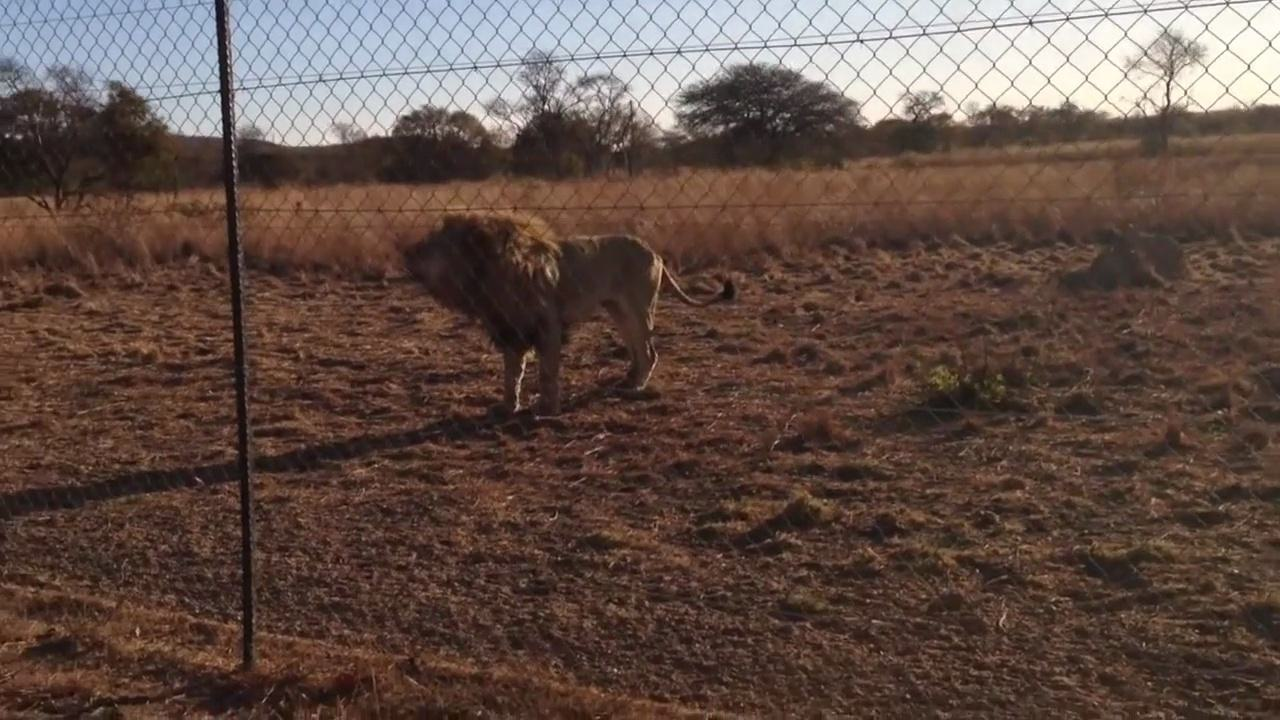
\includegraphics[width=1\linewidth]{1_img.jpg}
  %\caption{fig1}
  \end{minipage}%
  }%
  \subfigure[]{
  \begin{minipage}[t]{0.25\linewidth}
  \centering
  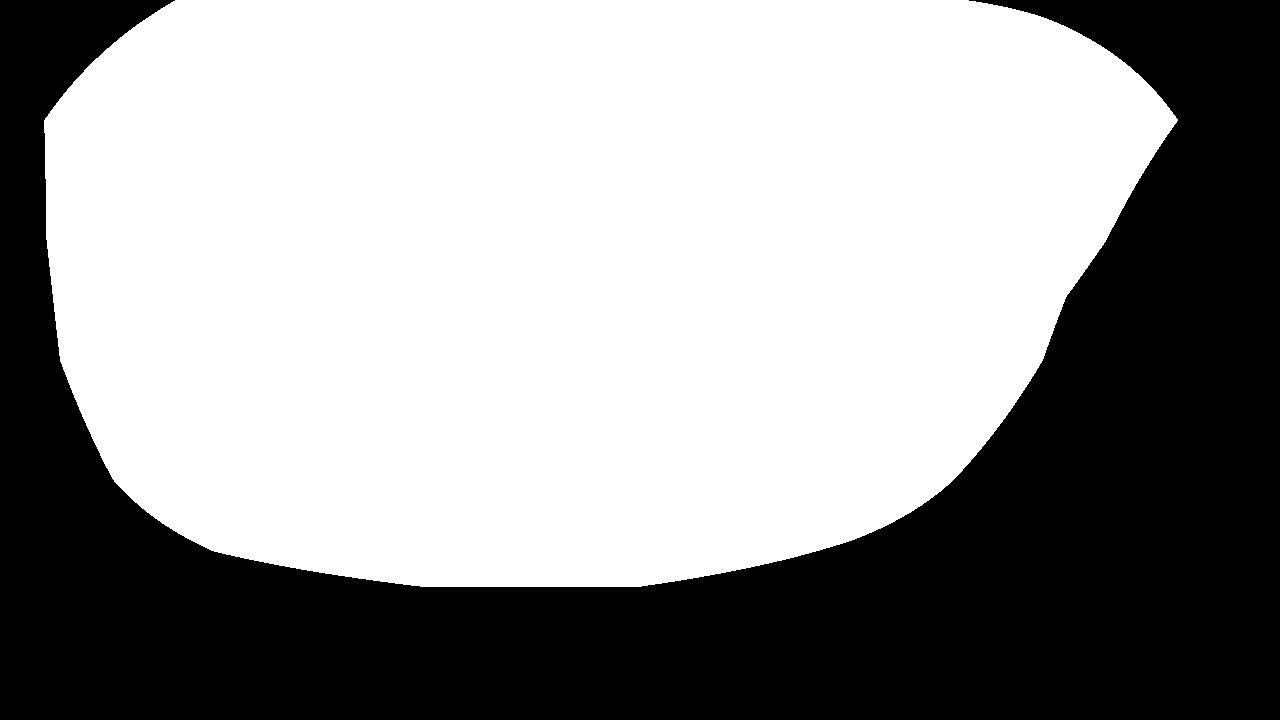
\includegraphics[width=1\linewidth]{1_avl_av_obj.jpg}
  %\caption{fig1}
  \end{minipage}%
  }%
  \subfigure[]{
  \begin{minipage}[t]{0.25\linewidth}
  \centering
  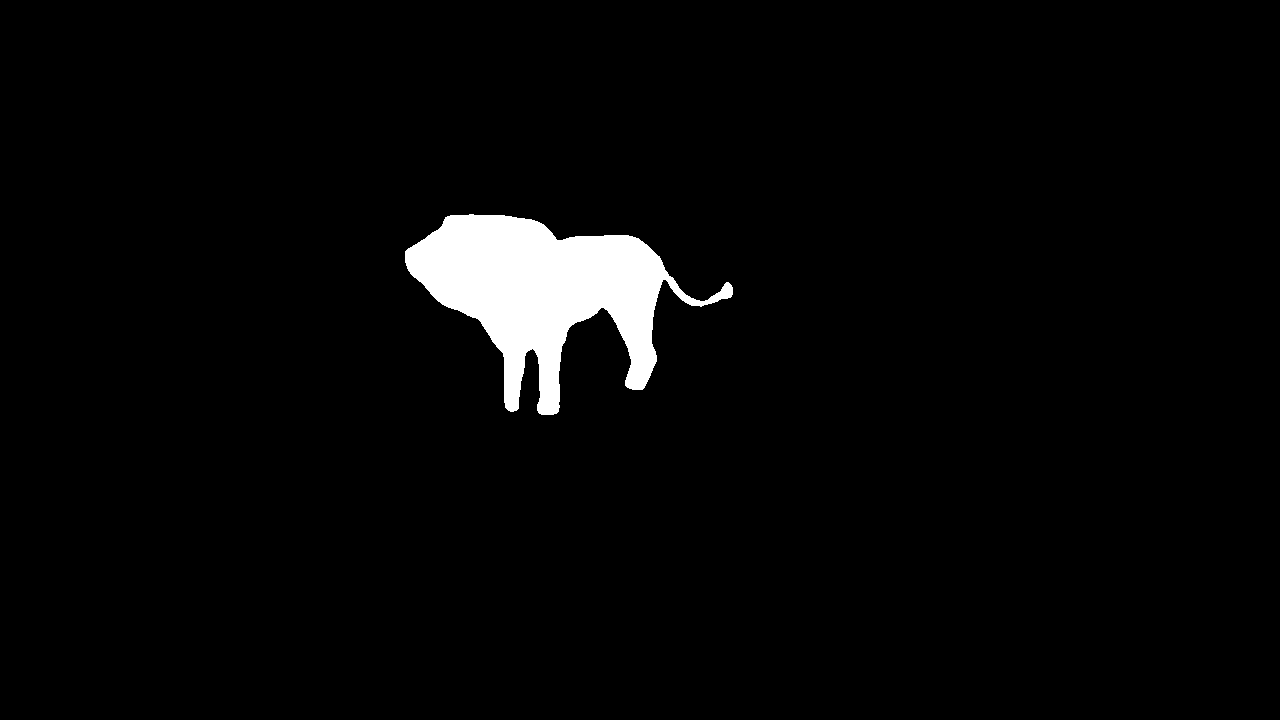
\includegraphics[width=1\linewidth]{1_avobj.png}
  %\caption{fig1}
  \end{minipage}%
  }%
  \subfigure[]{
  \begin{minipage}[t]{0.25\linewidth}
  \centering
  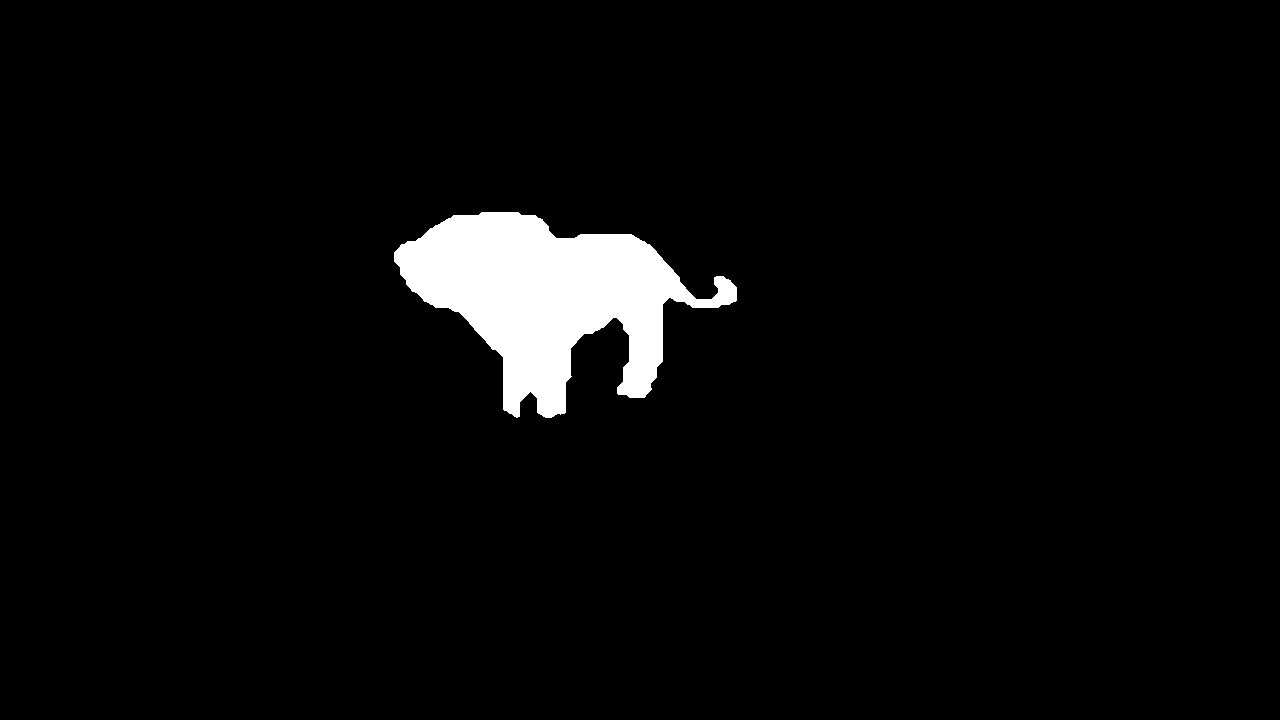
\includegraphics[width=1\linewidth]{1_gt.png}
  %\caption{fig1}
  \end{minipage}%
  }%

  \subfigure[]{
  \begin{minipage}[t]{0.25\linewidth}
  \centering
  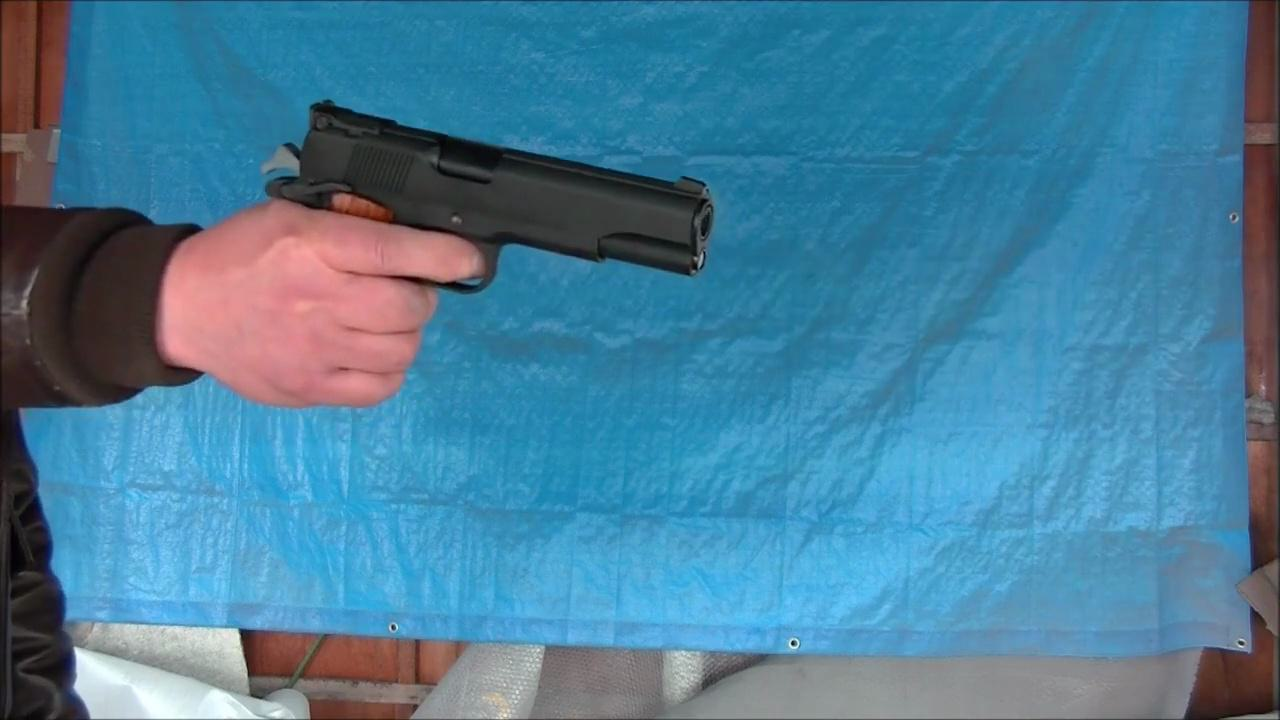
\includegraphics[width=1\linewidth]{26_img.jpg}
  %\caption{fig1}
  \end{minipage}%
  }%
  \subfigure[]{
  \begin{minipage}[t]{0.25\linewidth}
  \centering
  
\includegraphics[width=1\linewidth]{26_avl_av_obj.jpg}
  %\caption{fig1}
  \end{minipage}%
  }%
  \subfigure[]{
  \begin{minipage}[t]{0.25\linewidth}
  \centering
  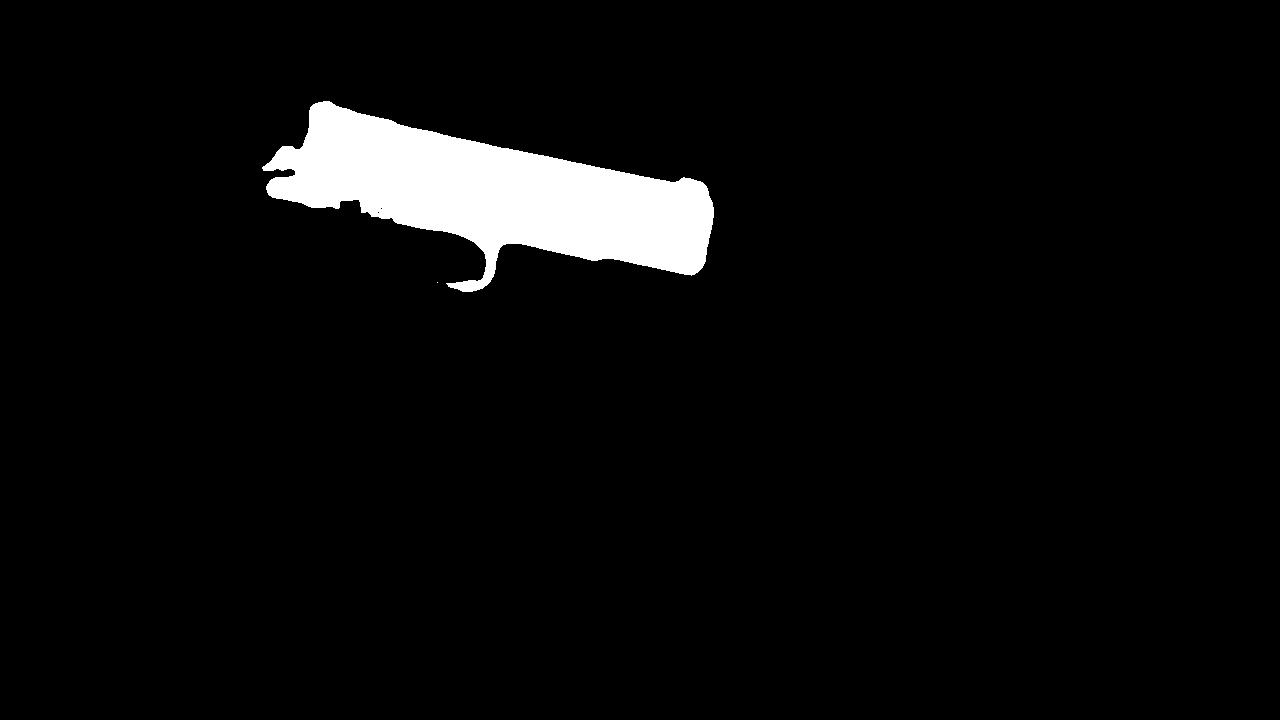
\includegraphics[width=1\linewidth]{26_avobj.png}
  %\caption{fig1}
  \end{minipage}%
  }%
  \subfigure[]{
  \begin{minipage}[t]{0.25\linewidth}
  \centering
  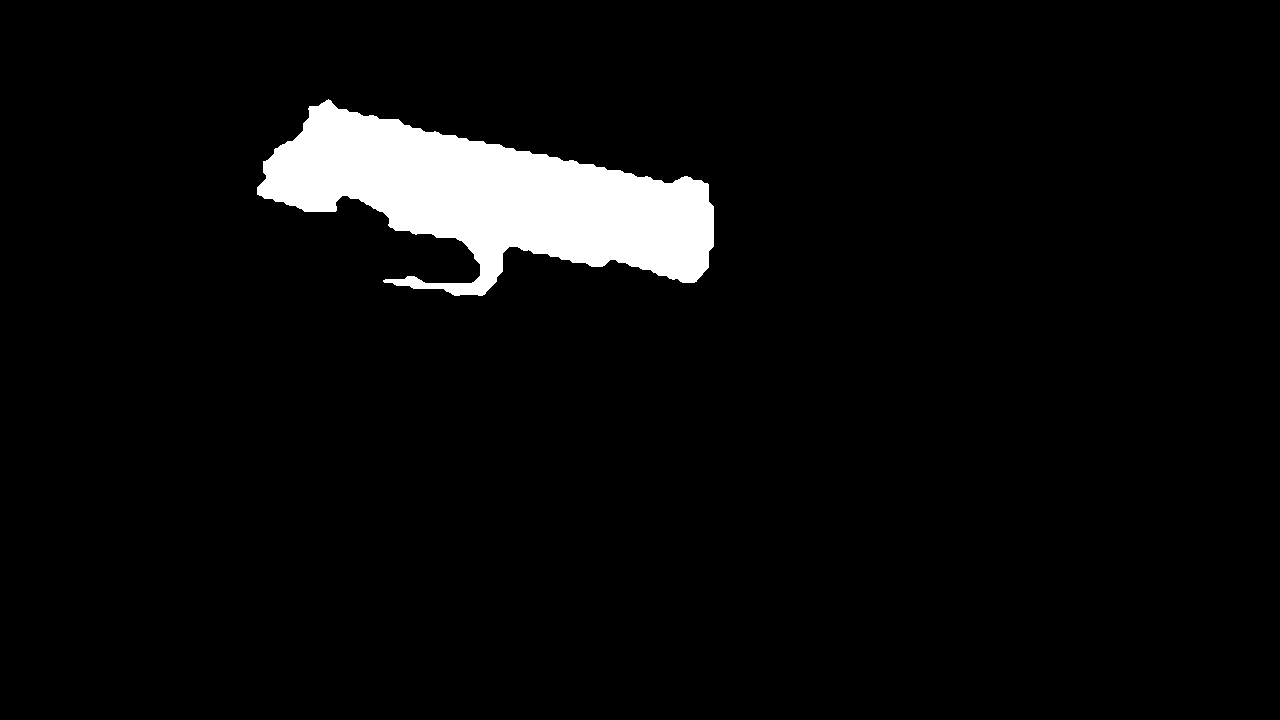
\includegraphics[width=1\linewidth]{26_gt.png}
  %\caption{fig1}
  \end{minipage}%
  }%

  \subfigure[]{
  \begin{minipage}[t]{0.25\linewidth}
  \centering
  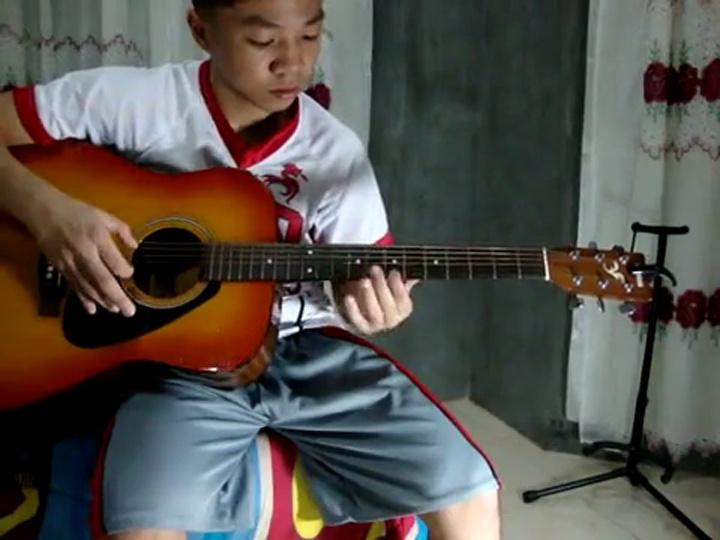
\includegraphics[width=1\linewidth]{29_img.jpg}
  %\caption{fig1}
  \end{minipage}%
  }%
  \subfigure[]{
  \begin{minipage}[t]{0.25\linewidth}
  \centering
  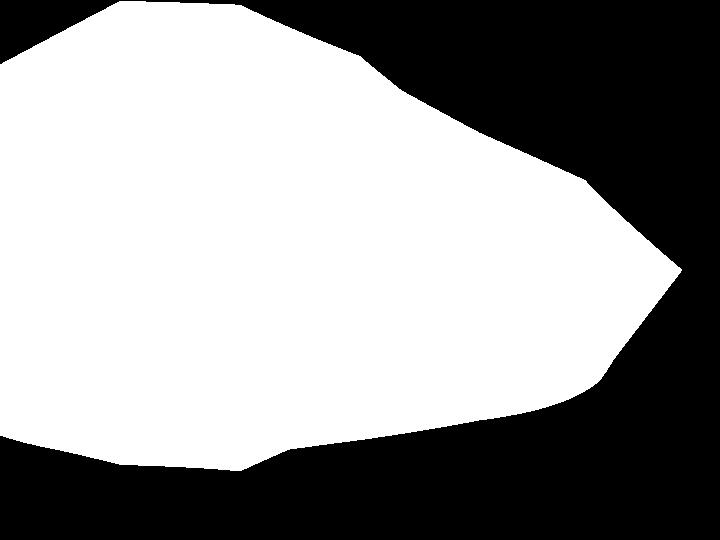
\includegraphics[width=1\linewidth]{29_avl_av_obj.jpg}
  %\caption{fig1}
  \end{minipage}%
  }%
  \subfigure[]{
  \begin{minipage}[t]{0.25\linewidth}
  \centering
  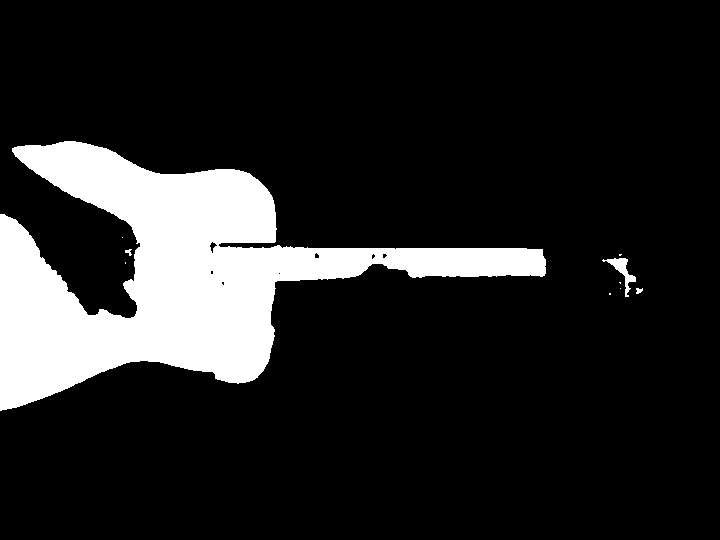
\includegraphics[width=1\linewidth]{29_avobj.png}
  %\caption{fig1}
  \end{minipage}%
  }%
  \subfigure[]{
  \begin{minipage}[t]{0.25\linewidth}
  \centering
  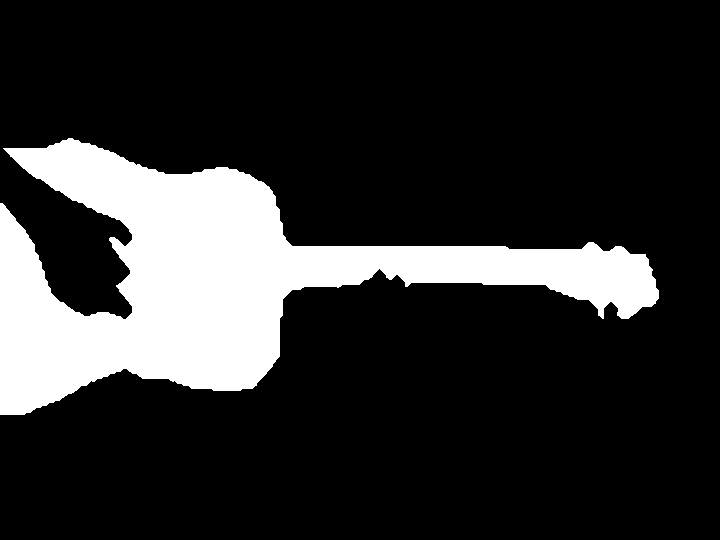
\includegraphics[width=1\linewidth]{29_gt.png}
  %\caption{fig1}
  \end{minipage}%
  }%
  \centering
  \caption{我们的方法与传统声源定位方法的效果对比。第一列为原图,第二列为EZVSL的结果,第三列为GSAVL的结果,第四列为掩码真值}
  \label{ref:res}
\end{figure}

出于对视觉和听觉这两种模态之间关联的兴趣,我们组选择了\textbf{声源定位任务(Sound Source Localization,SSL)},视听学习领域的重要任务之一,作为大作业的课题。声源定位任务使用未标记的视频样本进行训练,为输入音频定位视频帧中与声音相关的区域,结果通常以热力图呈现,通过音频特征和视觉特征的相似度矩阵得到,实现较细粒度的场景理解。视频数据中视觉和听觉特征在时间维度上的自然对应,为这个无监督任务的实现提供了可能,2018年牛津大学VGG组的工作\cite{object},首先提出视听对应方法(AVC),应用深度网络实现声源定位。在之后的几年里,涌现了许多优秀的工作,如引入对比学习的\cite{10},应用K-means聚类实现多声源定位的\cite{9},大大推动了视听学习领域的发展。

由于视频掩码标注的成本较高,声源定位任务在最初使用无标注视频进行训练,测试集的标注也仅为边界框标注而非掩码标注。这种无监督的任务设置,和测试集的评价指标,导致上述方法通常只能捕获粗略的物体轮廓。直到\cite{17}发布了具有像素级掩码注释的分割数据集,提出\textbf{声源分割(Audio-Visual Segmentation,AVS)}任务,旨在追求更细粒度的视听场景理解。该任务在过去一年里出现了两种主流方法,第一类为利用视觉基础模型SAM\cite{sam},加入视觉和听觉特征对齐进行微调\cite{s1,s6,s9},另一类为解耦语音特征,使用Mask2Former结构实现AVS\cite{s2,s3,s4}。值得注意的是,顶会ACM-MM在2023年的best paper便是视听分割领域的工作\cite{s10},相信该领域会在未来几年里激发社区更多优秀的工作。

正如上一段所说,\textbf{视觉基础模型SAM}已经被应用到视听学习领域,并取得优秀的表现。但是,据我们所知,目前还没有工作将SAM应用到声源定位任务中,我们小组希望借这次大作业的机会,将声源定位任务与SAM结合,在SSL无监督的任务设置下,实现具有强大零样本泛化能力、且具有分割粒度的声源定位模型,进一步探索SAM在视听学习领域的潜力。我们的课题与相关工作的区别与联系如图\ref{fig:01}所示。
\begin{figure}
    \centering
    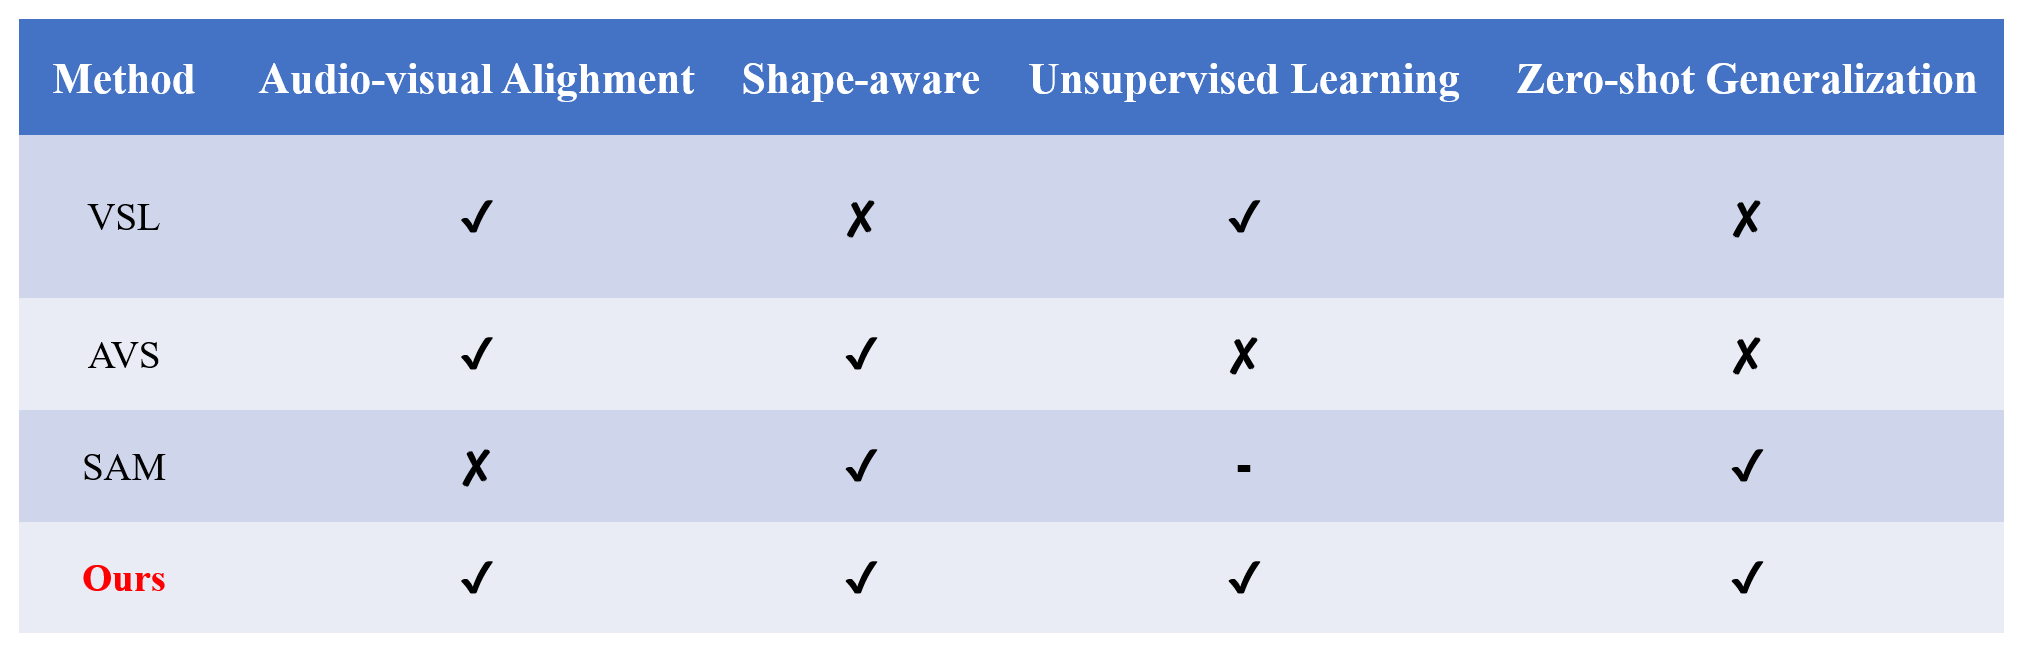
\includegraphics[width=1\linewidth]{label.png}
    \caption{我们的方法与其他相关工作的对比}
    \label{fig:01}
\end{figure}

为此,我们小组提出了\textbf{Generalizable Shape-aware Audio-Visual Localization(GSAVL)},模型结构如图\ref{refmodel1}所示。首先,我们基于EZ-VSL\cite{22},设计了一个更强大的声源定位模型,使用在大量语音数据上预训练的Vggish作为语音编码器,应用余弦相似度计算定位图,实现了更高的定位精度和泛化能力;其次,我们根据声源定位模型给出的模糊定位图,设计了高效采样器提取prompt;最后,我们将SAM加入整个pipeline,以提取的点作为prompt输入SAM,得到精确的声源预测掩码。

我们主要贡献如下:

\textit{i)我们进一步探索了视觉大模型SAM在audio-visual领域的潜力,将SAM应用到声源定位任务,提出GSAVL模型,在无监督设置下实现了像素级声源定位预测,在声源分割数据集AVSBench上效果远超传统的声源定位方法,相比30.22\%,我们实现了48.84\%的定位精度。}

\textit{ii)我们对EZ-VSL进行了改进优化,应用了一个更强大的语音编码器,并使用余弦相似度,在VGGSound数据集上的声源定位精度由36.67\%提升到37.23\%}

\textit{iii)我们基于prompt learning的思想,设计了几种高效的prompt采样器,在VGGSound数据集上验证了GSAVL强大的零样本泛化能力}
\section{相关工作调研}
我们小组将结合SAM大模型,在无监督设置下实现细粒度的声源定位。因此,我们在这一部分将分别讨论声源定位,SAM和声源分割的相关工作。

\textit{尽管该部分较长,但是均为小组成员阅读该领域论文后,将方法归类后总结而成,并非简单的流水账罗列,声源定位的论文笔记可见\href{https://github.com/ucasmjc/ruc-visiting/blob/main/SSL.md}{\faGithub},声源分割的论文笔记可见\href{https://numerous-jasmine-cee.notion.site/AVS-32583e7929274e4ba8d9e2c4c5a9cf17}{notion},写作过程中无AI使用。并且,由于声源定位领域并无综述,声源分割更是今年才出现的新任务,我们想复制也没有来源,希望我们的努力不会影响老师的评价。}
\subsection{声源定位}
声源定位任务是研究audio-visual learning的一个重要任务,近几年每年都可以在顶会上看到几十篇文章,但是,经过我们调研,目前存在的关于声源定位的综述,描述的是3维空间中的任务,与我们要探究的audio-visual领域的声源定位并无联系,而后者并未找到综述(至少我们没有查到)。因此,我们小组阅读了2018年以来声源定位领域的三十多篇顶会论文,论文笔记可见\href{https://github.com/ucasmjc/ruc-visiting/blob/main/SSL.md}{\faGithub},选择了其中的二十多篇经典论文,按照每篇文章的方法创新点,将它们分为以下四类,将在本部分分别讨论。
\subsubsection{Audio-Visual Correspondence}
利用语音-视觉一致性(AVC)进行SSL由\cite{object}首先提出,并一直作为SSL任务的训练目标之一延用至今。虽然SSL训练时的视频数据为无标注的,但视频数据自然地提供了语音和视觉特征沿时间维度的对齐,AVC方法便是为了利用这种自然对齐而提出的自监督方法。具体来说,分别提取同一秒的图片和声音数据的嵌入,让模型判断其是否对应,设计损失函数使相应视音对的预测值最大化,而最小化非相应对的预测。本文的模型方法如图\ref{ref1}所示,首先利用两个backbone分别提取14*14视觉特征图和一维全局语音特征,将二者逐点计算内积估计相似度,经过卷积块后,取sigmoid作为定位图,做最大池化作为“是否对应”的预测值。
\begin{figure}[!h]
  \centering
  \subfigure[]{
  \begin{minipage}[t]{0.15\linewidth}
  \centering
  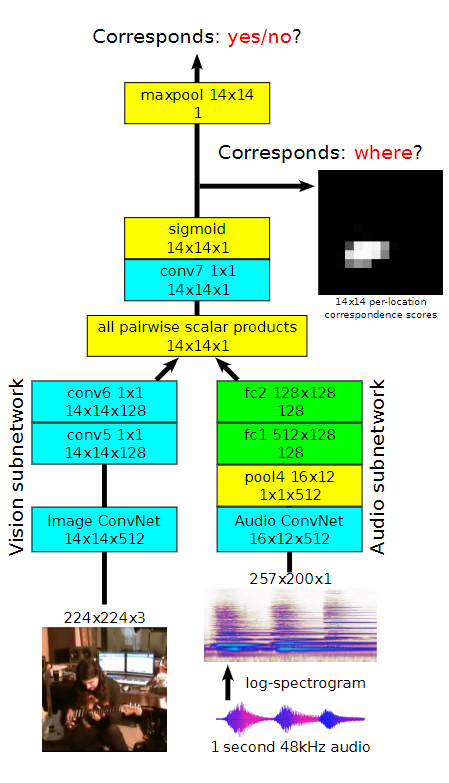
\includegraphics[width=1\linewidth]{1.png}
  %\caption{fig1}
  \end{minipage}%
  }%
  \subfigure[]{
  \begin{minipage}[t]{0.35\linewidth}
  \centering
  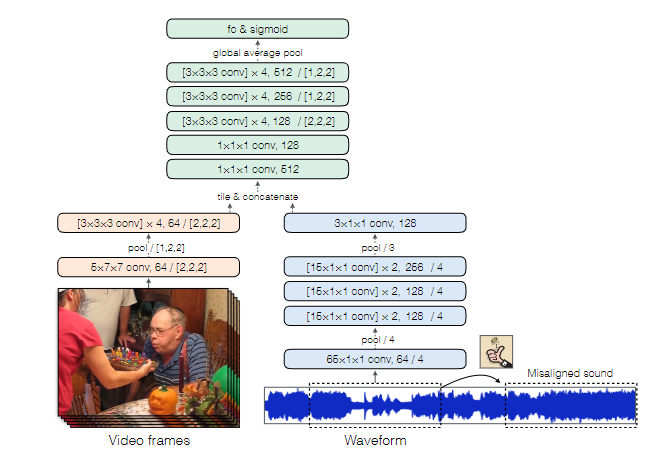
\includegraphics[width=1\linewidth]{2.png}
  %\caption{fig1}
  \end{minipage}%
  }%
  \subfigure[]{
  \begin{minipage}[t]{0.5\linewidth}
  \centering
  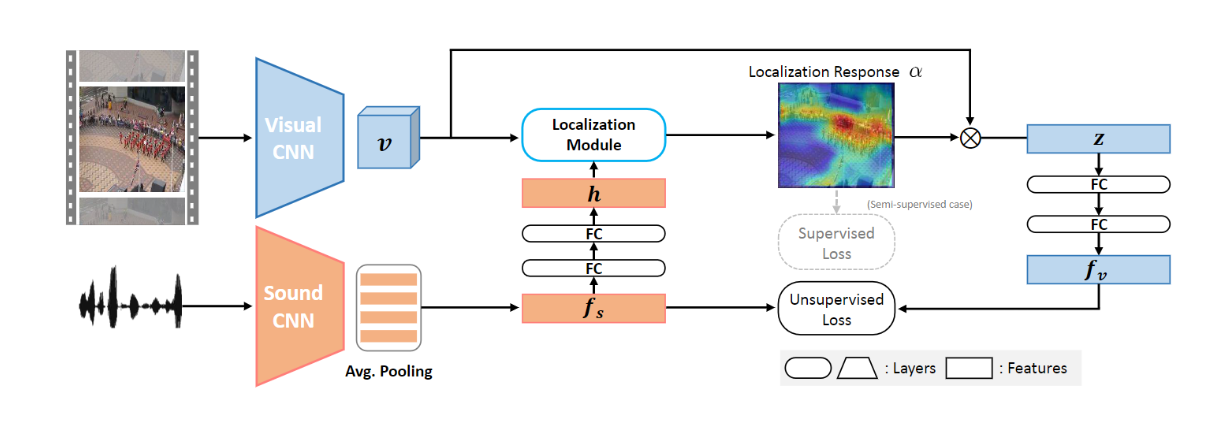
\includegraphics[width=1\linewidth]{3.png}
  %\caption{fig1}
  \end{minipage}%
  }%
  \centering
  \caption{(a)为\cite{object};(b)为\cite{ucb};(c)为\cite{6}}
  \label{ref1}
\end{figure}

UCB的\cite{ucb}也利用了AVC方法,如图\ref{ref1}所示。与前一篇工作的区别在于,本文为了利用时间维度的信息,输入模型的数据分别为连续的多帧图片和1维波形,视觉和语音backbone分别为3D和1D卷积,在得到相似度图后利用GAP得到判断对应的预测值,利用CAM得到定位图。

同为早期工作的\cite{6},提出了一种新的训练目标来捕捉AVC,如图\ref{ref1}所示。具体来说,在backbone提取的视觉和语音特征后加了几个非线性层,将两个模态的特征投影到同一特征空间,计算二者的L2距离作为损失,使相应视听对的L2距离拉近,非相应的拉远。

近几年,还有一些针对SSL中特定问题的工作,在AVC任务的基础上做了相应的提升。\cite{23}发现,目前的SSL模型在训练时极容易过拟合(这与我们的实验时的发现一致),于是给视觉特征加了0.9的dropout,并使用EMA(Exponential Moving Average)分别更新视觉和语音子网。\cite{23}认为目前的视觉特征未被充分利用,加入了视觉推理模块利用上下文语义信息,将视觉特征解耦。\cite{n2}认为之前工作为“强制对齐”两种模态的特征,于是提出了一个归纳模块,利用视觉模态引导音频模态的对齐,并发现利用停止梯度(stop-grad)解耦两种模态的梯度传播,可以显着提升视听表示的学习。\cite{n3}认为,当人看不见,只靠声音信息也能模糊的定位声源,因此语音信息也包含空间信息,同时人脑在定位目标时会递归地精确化位置,基于这样的直觉,本文计算了语音特征与视觉-语音融合特征的相似度图,与原相似度图线性相加,并加入了递归注意力模块。

\subsubsection{样本选择}
牛津VGG组的\cite{10}注意到SSL任务中的“难负例”(hard negative)样本,并引入了对比损失捕捉AVC,成为近年的主流方法。在过去的方法中,简单地将同一视频的图片帧和语音作为正例对,但是,一张图片中的非声源部分(背景)实际上与语音没有对应关系,是被忽视的难负例,让模型混淆。本文的动机便是挖掘难负例,设置阈值,将图片的像素分为背景、声源和模糊地带,如图\ref{ref2}所示。



在\cite{10}后,样本中的假负例(false negative),又称难正例(hard positive)也引起了广泛关注。该概念指的是,一个来自不同视频的图片-语音对,可能具有相似的语义信息,为同一声源对象,不应被判为“负例”,比如来自不同吉他视频的视音对,它们也应该被判定为正例,由此出现了一系列挖掘假负例(难正例)的工作。\cite{18}提出假负例会混淆模型的判断,于是提出了一种Negative-Free方法,只使用正例训练,引入孪生网络,并对正例进行数据增强。\cite{24}使用预训练backbone提取视觉和语音模态数据的特征,并在每一模态内部计算样本间的点积作为相似度,与自身前K相似的样本被视为正例,并进一步约束模态之间的正例对应。\cite{30}先计算模态内样本间的相似度矩阵,并以此作为AVC的软监督信号,即模态内特征相似的样本应具有更高的相应预测,如图\ref{ref2}所示,另外,本文还设计损失增强真负例的影响。

除此之外,还有一些改进对比损失的工作。\cite{21}通过在\cite{10}的对比损失中加入了一个负边界(margin),进一步抑制了假正例的作用。\cite{22}认为在没有精确声源位置信息的条件下,希望模型将语音表征和声源的视觉表征像素级对应是一个矛盾的问题,因此在对比损失中只要求语音特征响应视觉特征中最强的一个patch,做了一个模糊化处理,并且引入分类网络提供先验信息辅助定位,结构如图\ref{ref2}所示。


\begin{figure}[!h]
  \centering
  \subfigure[]{
  \begin{minipage}[t]{0.5\linewidth}
  \centering
  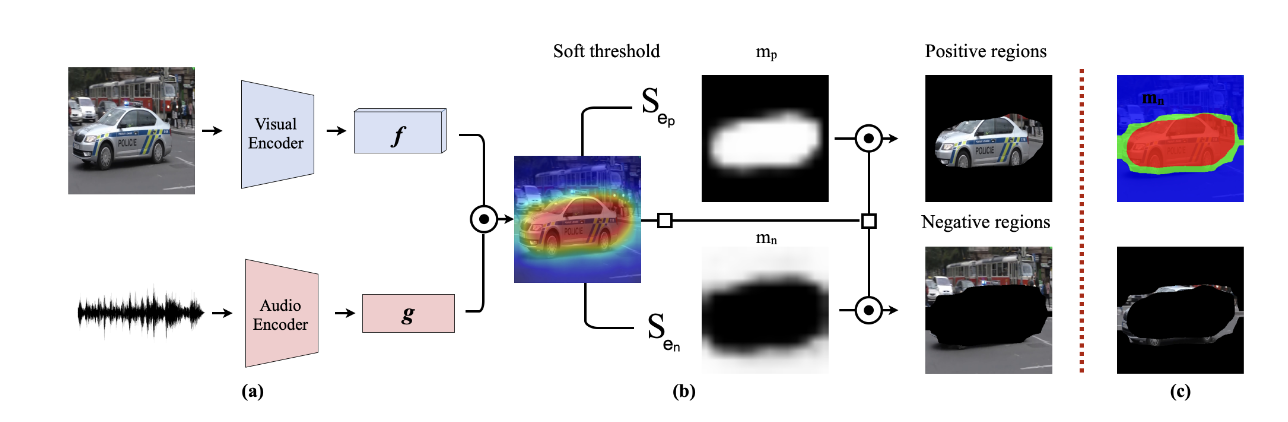
\includegraphics[width=1\linewidth]{4.png}
  %\caption{fig1}
  \end{minipage}%
  }%
  \subfigure[]{
  \begin{minipage}[t]{0.5\linewidth}
  \centering
  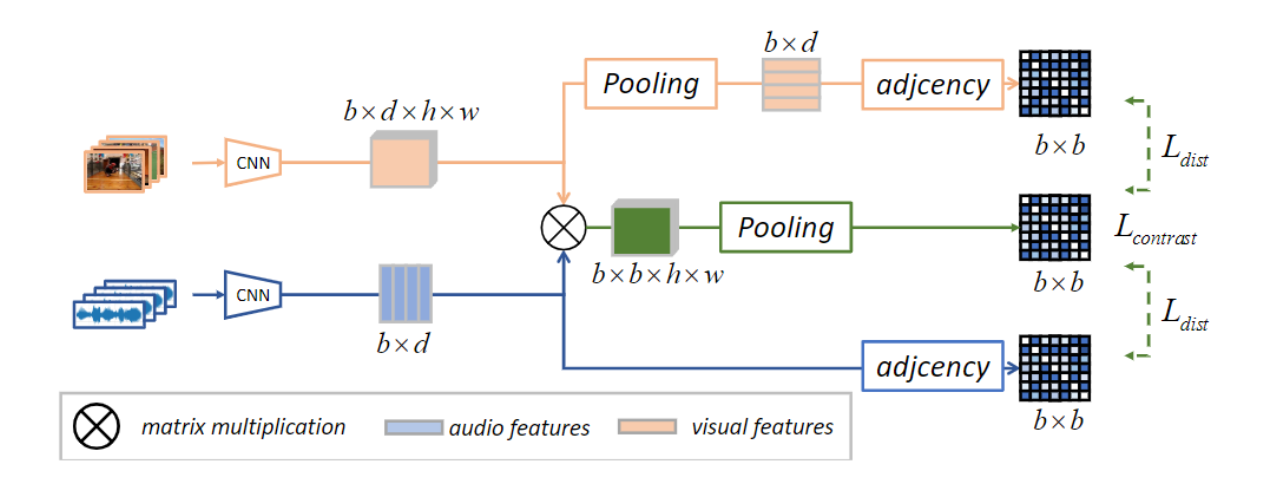
\includegraphics[width=1\linewidth]{5.png}
  %\caption{fig1}
  \end{minipage}%
  }%

  \subfigure[]{
  \begin{minipage}[t]{1\linewidth}
  \centering
  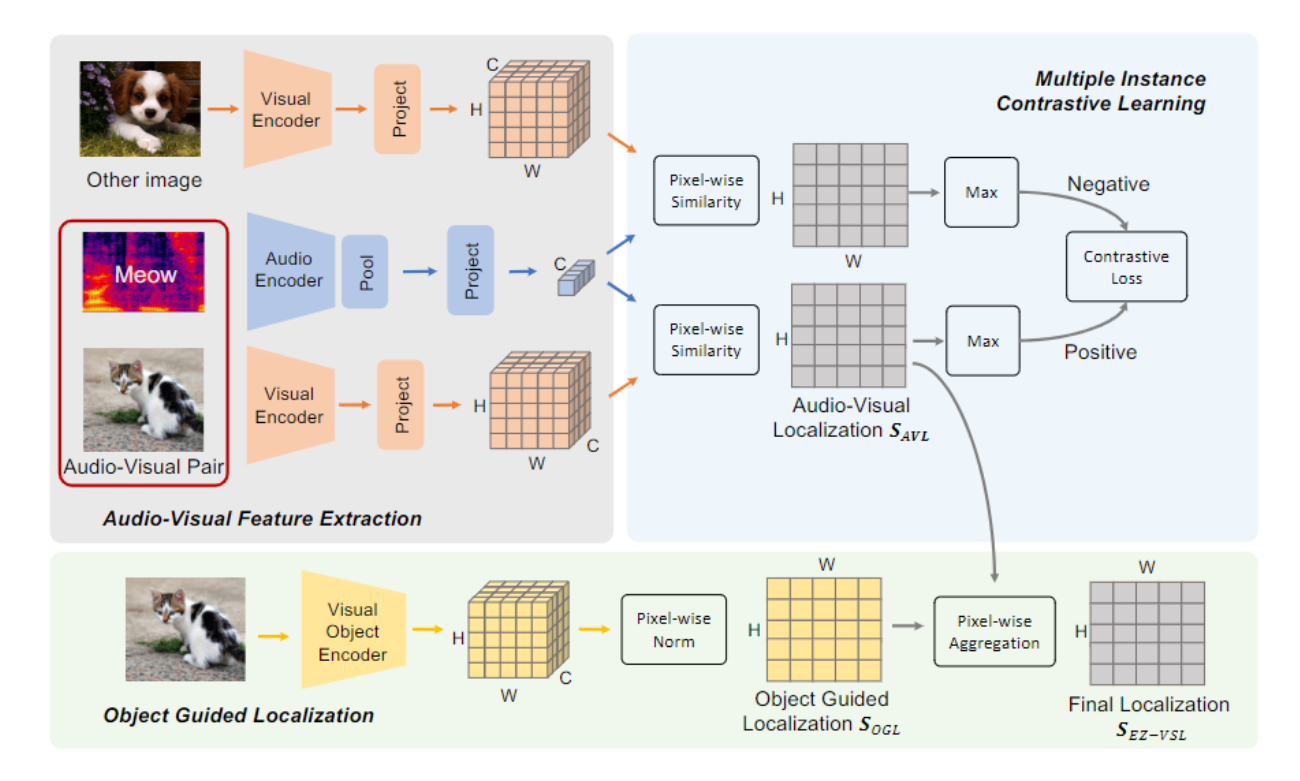
\includegraphics[width=1\linewidth]{6.png}
  %\caption{fig1}
  \end{minipage}%
  }%
  \centering
  \caption{(a)为\cite{10};(b)为\cite{30};(c)为\cite{22}}
  \label{ref2}
\end{figure}

\subsubsection{解耦图片和语音特征}
AVC方法根据视频级别的同步,利用音频和视觉信号是否源自同一视频的对应关系实现声源定位,这对于简单场景(单声源)有效,但在现实世界中,各种声音通常混合在一起,而视频级自监督过于粗糙,难以提供每个声音和视觉源对之间的精确对齐。因此,出现了一系列按语义将图片和语音特征解耦并对齐的工作,在多声源定位任务中表现出强大的性能。

早期工作\cite{4}使用CNN提取图片的K张特征图,用Audio U-Net提取音频的K张特征频谱图,用前者每个像素的特征加权K张频谱图,从而得到论文名字中的“每个像素的声音”,最终通过聚类定位声源。\cite{7}是\cite{4}的延续,为了适应现实情况(不一定总为有同步音频的视频),可以在只输入图片的情形下输出对应类别的分割图,在只输入混合音频时输出分离的声音。

以显示或隐式解耦视觉和语音特征的类别信息,成为多声源定位的经典方法。\cite{9}认为视频中混合的多个视觉对象和声音,使得在无监督环境中执行有效的匹配变得困难,于是引入K-means聚类,提出了深度多模态聚类(Deep Multimodal Clustering)方法,建立视听聚类中心来分解混合输入的语义,并建立模态间聚类中心的对应关系。但是,\cite{9}需要预先确定聚类中心的数量,这在无约束的现实场景中变得困难,极大地影响对齐性能,\cite{11}提出一个两阶段训练框架,由粗到细的实现多声源定位,第一个阶段以分类(用到了数据集的image-level标注)和对应(AVC)为目标任务训练视觉和声音的对齐,第二阶段利用grad-CAM得到视-音每个类别的特征表示,并
用L2损失对齐两个模态类别级别的特征表示,如图\ref{ref3}所示。\cite{11}在进行类别对齐时,按数据集设置类别数量,这在真实场景下是不可知的,\cite{12}进行了扩展,在训练时设置了潜在类别,将训练数据集分为单源和多源两类,第一阶段在单声源的视音对上训练,
用较简单的样本构建潜在类别表示的字典,在第二阶段用复杂的多声源样本训练,用构建的词典预测图片中潜在的发声对象,并要求发声对象的视觉类别分布与混合声音的类别分布相匹配,结构如图\ref{ref3}所示。

近两年,还有一些应用新方法的工作。\cite{25}针对真实视听声源定位的噪声问题,如图片中的声源目标不发出声音,或者声源在屏幕之外,或者混合
音频中音量大的会起主导作用,在\cite{12}的基础上加入interference eraser消除噪声影响。\cite{31}提出一个Transformer结构,输入N个可训练的类别token,实现视觉和语音特征的解耦。


\begin{figure}[!h]
  \centering
  \subfigure[]{
  \begin{minipage}[t]{0.5\linewidth}
  \centering
  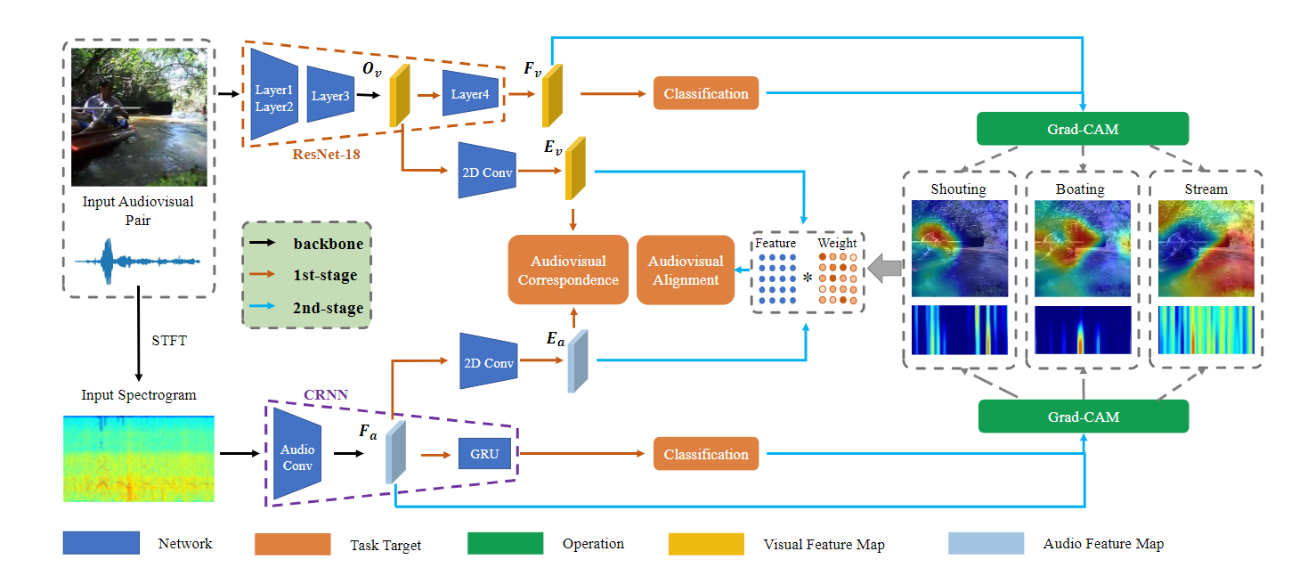
\includegraphics[width=1\linewidth]{7.png}
  %\caption{fig1}
  \end{minipage}%
  }%
  \subfigure[]{
  \begin{minipage}[t]{0.5\linewidth}
  \centering
  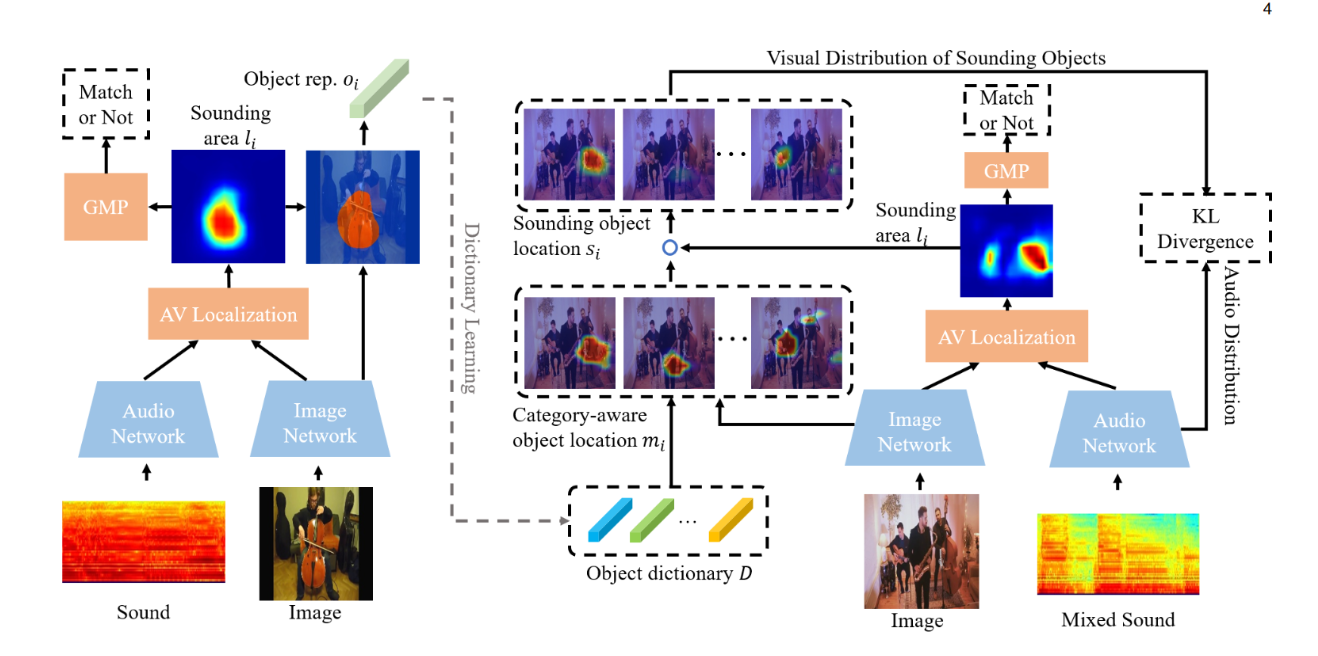
\includegraphics[width=1\linewidth]{8.png}
  %\caption{fig1}
  \end{minipage}%
  }%
  \centering
  \caption{(a)为\cite{11};(b)为\cite{12}}
  \label{ref3}
\end{figure}
\subsubsection{时间维度}
基于“视频中移动的物体往往是声源”这样的直觉,利用视频的时间上下文可能会有助于提高声源定位的性能,由此出现了一些利用时间维度信息的方法。\cite{8}基于\cite{4}的框架,将视觉子网换为动作子网,输入连续的图片帧,先用PWC-Net预测光流,再根据密集光流迭代地预测密集轨迹,最后用CNN提取轨迹特征,明确建模动作信息,实现声音的定位和分离,如图\ref{ref4}所示。\cite{28}在\cite{10}的基础上加入了光流定位子网,融合了时间尺度信息,对定位图进行修。\cite{33}提出了三种在SSL应用光流的方法,分别是直接将预测的光流和原定位图相乘、将视觉编码器增加一个光流通道(输入RGB+光流)和增加一个光流编码器,取得了不错的结果。
\begin{figure}[!h]
  \centering
  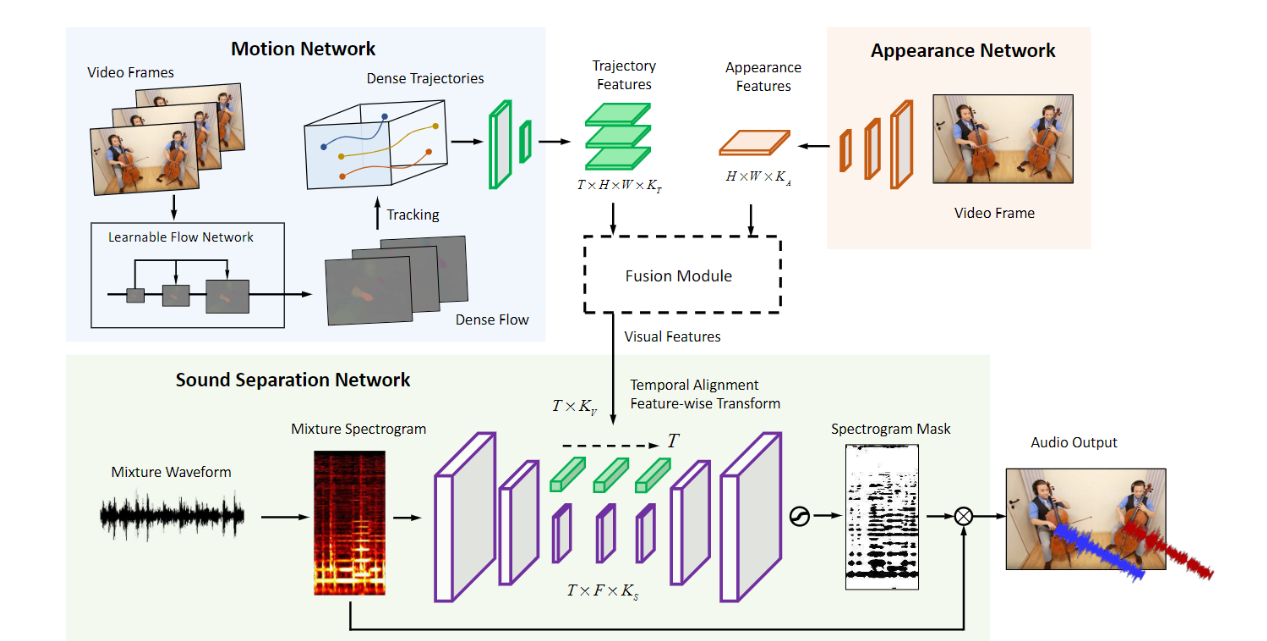
\includegraphics[width=0.7\linewidth]{9.png}
  %\caption{fig1}
  \caption{\cite{8}}
  \label{ref4}
\end{figure}

\subsection{Segment Anything}

继ChatGPT在NLP领域掀起大模型的热潮,Segment Anything\cite{sam}作为计算机视觉社区中第一个图像分割大模型发布,该模型使用超过 1100 万张图像和掩码进行预训练,支持多种提示(包括点、框、掩码和文本),具有强大的零样本泛化能力和令人印象深刻的视觉分割效果,很快被用来解决各种视觉问题,其主要结构如图\ref{ref6}所示。在视听声源分割领域,目前出现了AV-SAM\cite{s1},GAVS\cite{s6},SAMA-AVS\cite{9}等工作,揭示了SAM在该领域的强大潜力,但很少有工作探索 SAM 用于视听定位任务。因此,我们的项目为 SSL任务提出了一种基于 SAM 的模型,借助其强大的分割和零样本泛化能力,我们的模型实现了无监督设置下的具有强大零样本泛化能力,且可以预测目标形状的声源定位。
\begin{figure}[!h]
  \centering
  \centering
  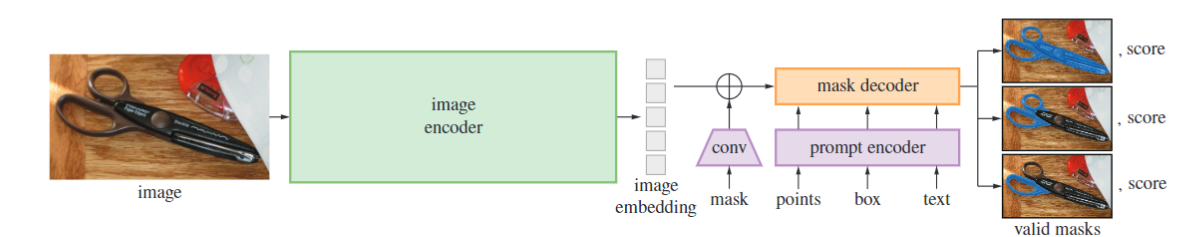
\includegraphics[width=1\linewidth]{12.png}
  %\caption{fig1}

  \caption{Segmenta Anything\cite{sam}}
\label{ref6}
\end{figure}
\subsection{视听分割(Audio-Visual Segmentation,AVS)}
SSL在无监督设置下,希望利用视觉和语音特征的自然对应关系进行视频理解,通常预测一个热力图来给出声源的位置,而无法考虑声源的实际形状。直到\cite{17}在2022年提出了视听分割(AVS)任务,该任务要求模型在监督学习的设置下密集地预测每个像素是否对应于给定的音频,从而生成声源的精确定位掩码,并开源了第一个像素级视听分割数据集 AVSBench,为声源提供GT掩码标注。在过去一年里引出许多工作,2023 ACM-MM的best paper\cite{s10}便是视频视听分割的工作,相信会在未来一年引起更多MM社区的关注。

经过我们小组调研,AVS近一年的工作主要可以分为两种方法,下面将分别介绍。

基于SAM\cite{sam}的方法.AV-SAM\cite{s1}利用语音子网提取语音特征,并将其与SAM图片编码器提取的视觉特征融合,得到的多模态融合特征代替图片特征输入SAM的mask decoder,经训练微调后实现声源分割。GAVS\cite{s6}为了增强AVS模型的泛化能力,融合语音特征和视觉特征作为prompt,并在SAM的mask decoder加入adapter,在AVS数据集上训练得到具有强大零样本泛化能力的模型,结构如图\ref{ref5}所示。SAMA-AVS\cite{s9}尝试将音频信息注入到图像特征中,在SAM的图片编码器每一层后加入adapter,将经过adapter的语音特征与图片特征相加,输入下一编码块,以实现视听表示的深度融合,在训练时,只微调adapter和mask decoder的参数。
\begin{figure}[!h]
  \centering
  \subfigure[]{
  \begin{minipage}[t]{0.5\linewidth}
  \centering
  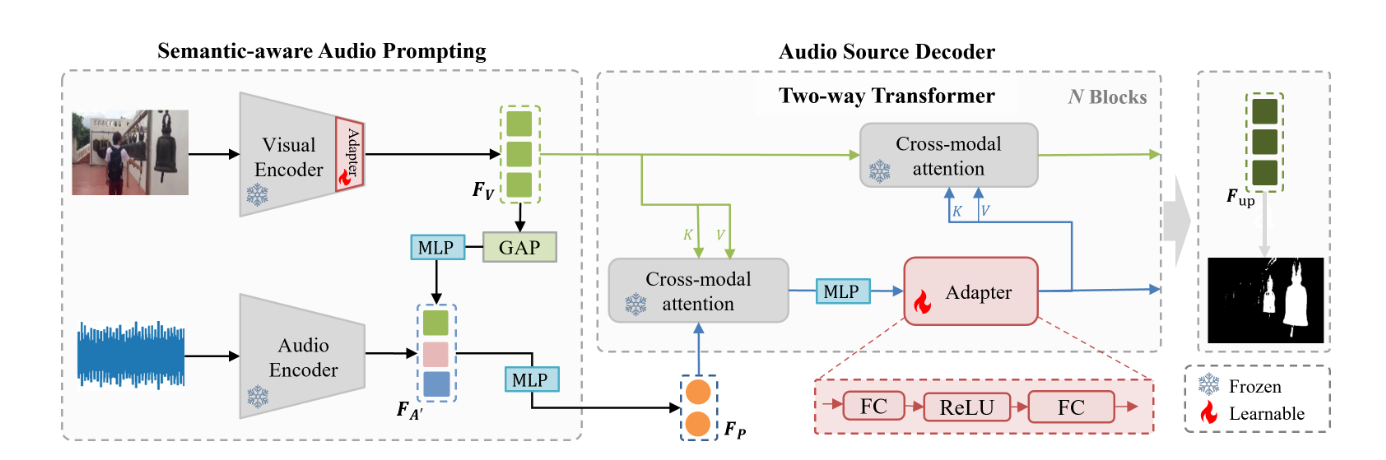
\includegraphics[width=1\linewidth]{10.png}
  %\caption{fig1}
  \end{minipage}%
  }%
  \subfigure[]{
  \begin{minipage}[t]{0.5\linewidth}
  \centering
  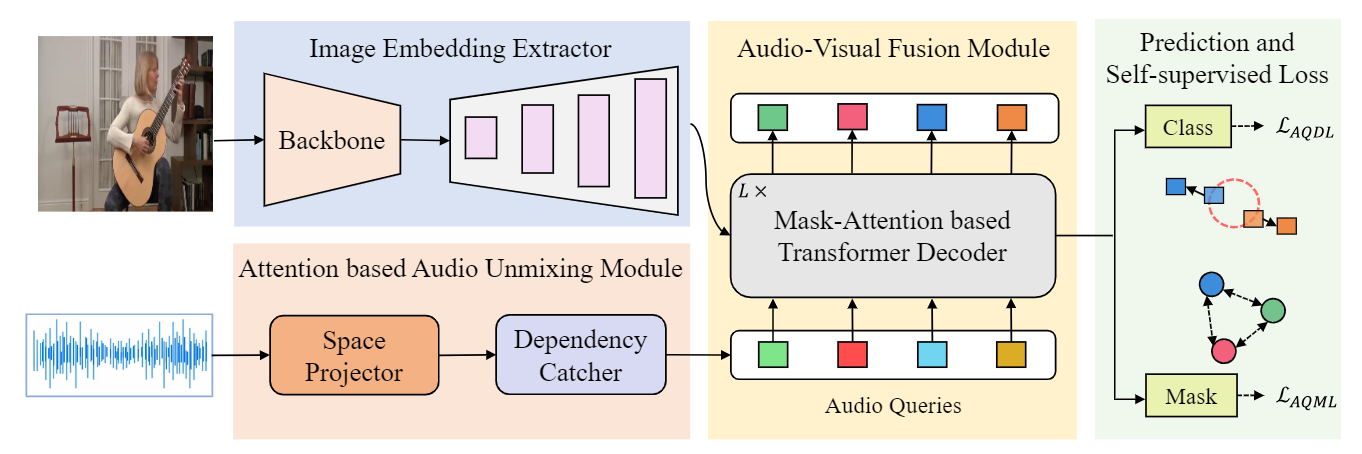
\includegraphics[width=1\linewidth]{11.png}
  %\caption{fig1}
  \end{minipage}%
  }%

  \caption{(a)为GAVS\cite{s6};(b)为AUSS\cite{s2}}
    \label{ref5}
\end{figure}

借鉴了Mask2Former\cite{mask}思想的语音解耦方法。AUSS\cite{s2}将语音特征扩展后,作为query输入Transformer解码器,并在其中与部分视觉特征融合,以最后一层特征图为掩码特征,将融合后的query与掩码特征做点乘,得到对应二元掩码,为了保证audio query的异质性,文中还引入了两种辅助损失,得到了很好的效果,保持了很久的sota,网络结构如图\ref{ref5}所示。AVSegFormer\cite{s3}、AuTR\cite{s4}方法类似,将视觉特征经过了transformer encoder融合多模态特征,并以多模态融合特征为掩码特征。
AQFormer\cite{s7}的掩码特征融合了时间上下文;SQD\cite{s8}引入product quantization方法对语音进行解耦,实现从视频到帧的细化的语义理解。CATR\cite{s10}在编码器全面地融合视觉-语音特征,利用门控模块融合不同时间步的特征,还引入视频分割的预训练模型提供先验信息。

除了上述两种方法,还有一些其他工作。AVSBench\cite{17}应用语义分割经典的编码器+融合+解码器结构,在融合的每个阶段加入语音特征;AVSC\cite{32}与语音解耦的方法类似,但是是将视觉对象解耦,向mask decoder输入对象query,得到每个对象类的二元掩码,将语音特征经过全连接层后按类别加权二元掩码得到最终预测;ECMVAE\cite{s11}从有效表示学习的角度,提出显式条件多模态VAE,得到了不错的表现。



\section{方案}
给定一段包含声源的视频,我们的目标是在不使用其他人工注释的设置下进行训练,定位其中的声源,并可以预测出声源的形状。为此,我们结合视觉大模型SAM提出了一种简单而有效的无监督声源定位方法,整个pipeline为“声源定位+prompt采样+SAM”,将其表示为GSAVL。我们将在\ref{encoder}介绍特征编码器,在\ref{loss}介绍对齐视觉和音频特征的方法,并给出实现自监督的损失函数形式,在\ref{sampler}介绍模型进行提示学习的方法,在\ref{sam}介绍Segment Anything的作用。整体结构如图\ref{refmodel1}所示。
\begin{figure}[!h]
  \centering
  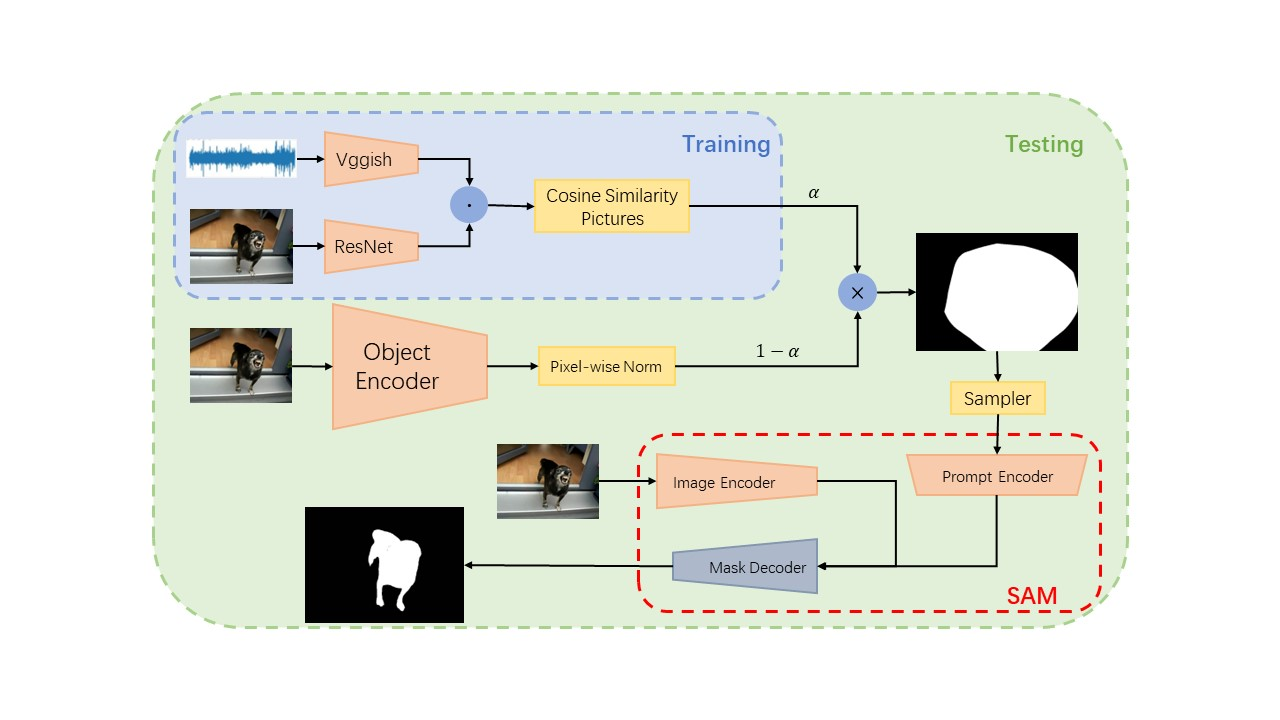
\includegraphics[width=1\linewidth]{model2.jpg}
  %\caption{fig1}
  \caption{GSAVL整体结构}
    \label{refmodel1}
\end{figure}
\subsection{单模态特征提取}\label{encoder}
以$D={(v_i,a_i):i=1,...,N}$表示配对的图片和音频的数据集,其中每一对的图片$v_i \in R^{3*H_v*W_v}$来自视频的第一帧图片,音频$a_i \in R^{T*H_a*W_a}$由原始的一维声波通过短时傅里叶变换(STFT)转换为二维声谱图(在代码中与此略有不同),从而可以使用CNN来提取音频模态特征。

具体来说,对于音频数据,我们以在大型音频数据集上预训练的VGGish\cite{vggish}作为音频编码器,将提取的$\widetilde{f_a}\in R^{T*C_a}$沿时间维度均值池化,并线性映射到与视觉共享的特征空间,得到$f_a \in R^c$。对于图片输入,我们使用经过预训练的ResNet18作为视觉编码器,得到视觉特征图$f_v \in R^{c*h*w}$。
\begin{figure}[!h]
  \centering
  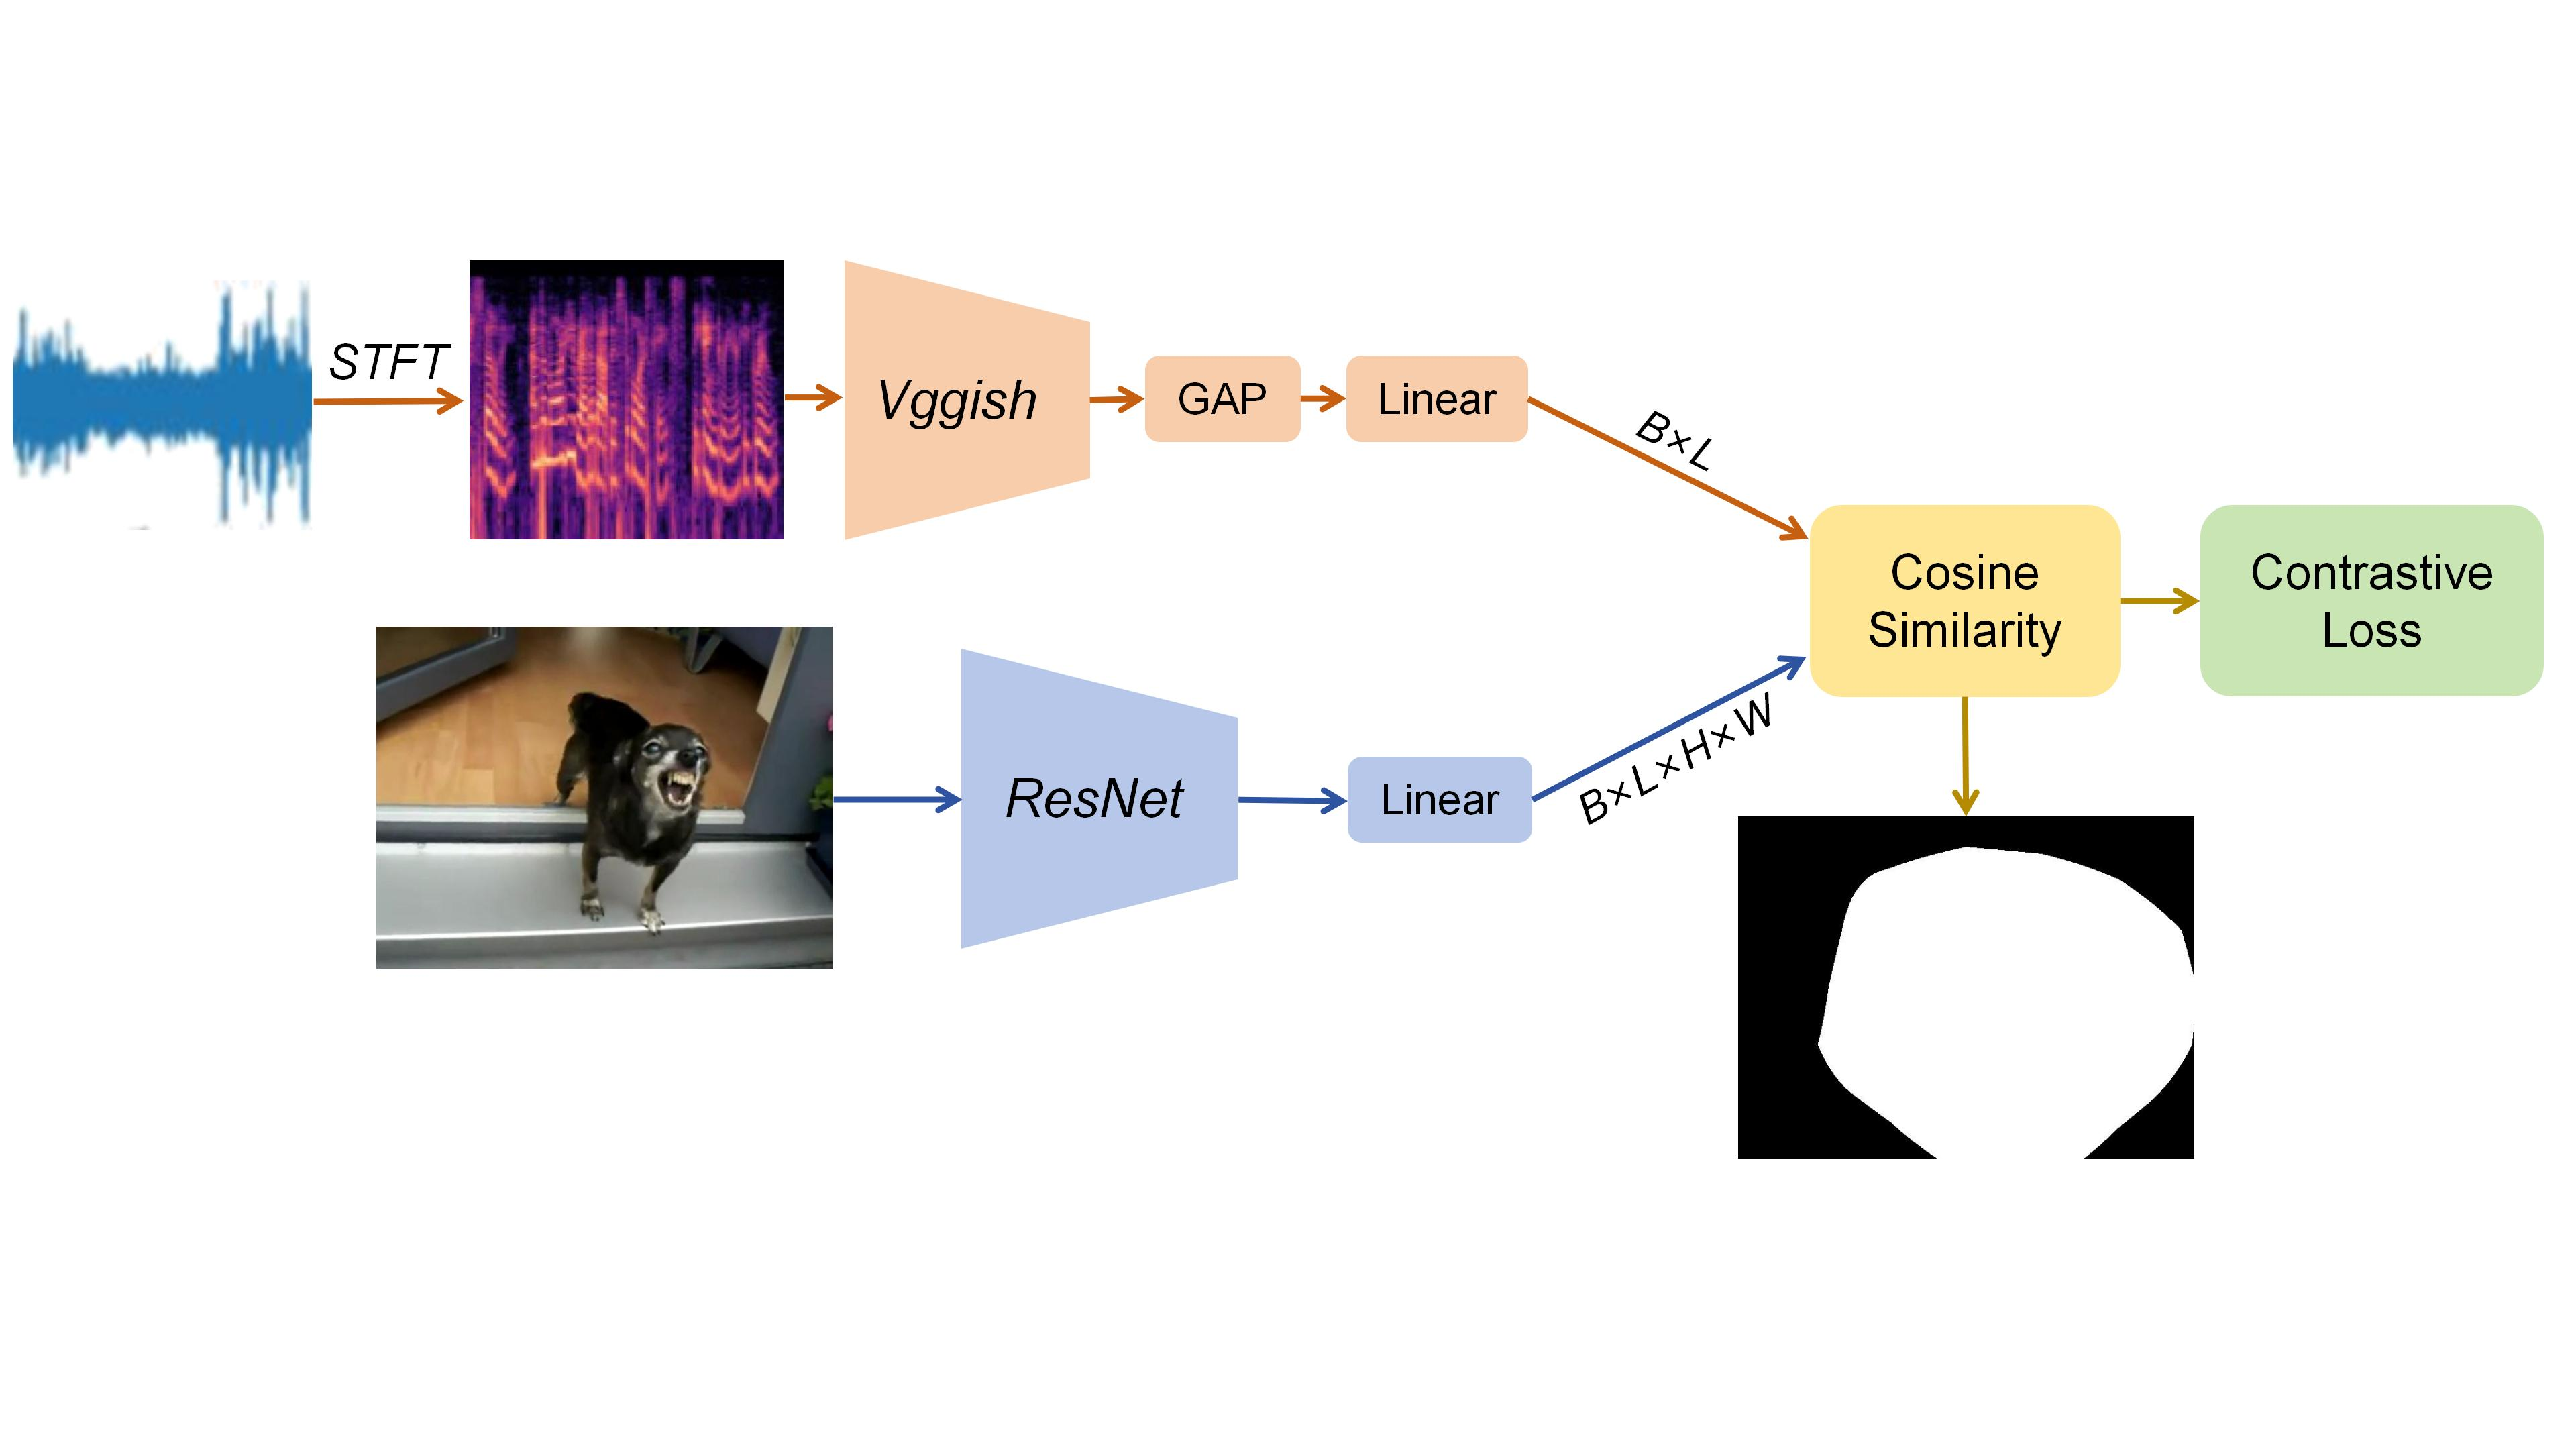
\includegraphics[width=1\linewidth]{model1.jpg}
  %\caption{fig1}
  \caption{声源定位模型整体结构}
    \label{refmodel2}
\end{figure}
\subsection{视觉-音频匹配}\label{loss}
我们遵循之前的工作\cite{10,22},根据视觉表示和音频表示的相似性引导视觉和音频的匹配,并以此作为定位图。对于来自同一个视频的图片和音频,我们希望模型认为它们是对应的,编码的视觉和音频特征具有更高的相似性,对于来自不同视频的图片和音频,希望他们编码的特征不相似。同时,为了降低模型的歧义性,我们只要求模型将音频特征匹配图片中最相似的一个部分,\cite{22}证明了该方法的有效性。

具体来说,我们采用余弦相似度(或归一化内积)来衡量音频和视觉特征之间的相似度,形式上,第i个样本的音频特征与第j个样本的视觉特征相似度计算如下
\[S_{ij}(x,y)=\frac{<f_a^i,f_v^j(x,y)>}{\Vert f_a^i\Vert \Vert f_v^j(x,y) \Vert}\]
我们使用对比损失引导模型学习到视音对应,对于一个批次的数据,我们将相应视音对的音频和最相似的图片部分作为正例,同一批次非相应视音对的音频和最相似的图片部分为负例,音频对视觉的对比损失形式如下,
\begin{equation}
L_{a->v}^i=-log\frac{exp(\frac{1}{\tau}\mathop{\max}_{x,y}(S_{ii}(x,y))}{\mathop{\sum}_{j}exp(\frac{1}{\tau}\mathop{\max}_{x,y}S_{ij}(x,y))}
\end{equation}
其中,$\tau$为温度超参数,负例j来自同一批次的其他样本。在训练时,我们还加入了一个对称形式的损失,
\begin{equation}
L_{v->a}^i=-log\frac{exp(\frac{1}{\tau}\mathop{\max}_{x,y}(S_{ii}(x,y))}{\mathop{\sum}_{j}exp(\frac{1}{\tau}\mathop{\max}_{x,y}S_{ji}(x,y))}
\end{equation}
总损失为
\[L=L_{a->v}+L_{v->a}\]
\subsection{视觉对象定位}
在声源定位中,有一些视觉的先验信息可以被利用,比如蓝天白云不会是声源,声源一般为图片中的显著对象。因此,在推理时,我们提出了一种视觉对象指导的方案,利用预训练视觉backbone中的先验信息来增强定位效果。

遵循先前的工作\cite{22},我们使用在ImageNet上预训练的ResNet18,去掉最后的全局池化层和全连接分类头,而直接利用最后的激活图$f_{obj} \in R^{c*h*w}$ 。该模型与用于声源定位的视觉编码器具有相同的架构,并使用相同的 ImageNet 预训练权重进行初始化,但与前者不同的是,该模型从未针对视听相似性进行训练。因此,特征图$f_{obj}$不包含有关音频的信息,可以用于提供场景中的视觉对象的定位先验,无论这些对象是否是声源。由于ResNet是基于对象级别的分类任务进行的预训练,在图像进行推理时会在对象附近产生更强的激活,因此我们直接使用L1正则化后的激活图作为视觉对象定位图,
\[S_{obj}=\Vert f_{obj} \Vert_1\]
最终的定位预测图,由\ref{loss}中声源定位模型得到的声源预测和视觉对象定位图线性组合得到,
\[S=\alpha S_{ssl}+(1-\alpha)S_{obj}\]
\subsection{提示学习}\label{sampler}
近年来,预训练大模型的表现令人印象深刻,如何在下游任务里更好地利用预训练模型的先验知识成为人们关注的重点。得益于这些模型的参数量足够大、训练过程中使用了足够多的数据、同时设计的预训练任务足够有效,一些工作发现,Prompt learning所带来的增益远远高于标准的Finetuning,通过提供特定于任务的线索来协助模型有效地利用预训练时学到的知识,只需要设计合适的指令模板即可以适应下游任务,小样本甚至是零样本的性能也能够极大地被激发出来。prompt learning的一些经典方法,比如上下文学习 In-Context Learning、指令学习 Instruction-tuning和思维链 Chain-of-Thought(CoT)。

在前三个部分,我们阐述了如何训练出一个优秀的声源定位模型,在这一部分,我们将解释如何基于声源定位模型的结果进行提示学习,得到精确、鲁棒的提示,指导SAM进行对声源对象的精确定位。
%第二段可以改一下说法,下面几个采样器,不用提每一个的具体效果(不好),比如“朴素采样器效果不行”之类的,可以说“为了提高提示学习的鲁棒性,我们还尝试了……”
%定位特征图由S表示,采样出来的点由$f_p$表示
\subsubsection{朴素采样器}
朴素采样器为最直接的实现方式,对于声源定位模型预测的定位图S,上采样后使用'np.argmax'函数找到S中具有最大权重值的像素点$f_p$的位置,再使用'np.unravel\_index'函数将该索引转换为对应的行列坐标即可,
$$f_p=argmax_{x,y}S(x,y)$$

朴素采样器的优点是简单易实现且计算效率较高,在声源较大,声源定位模型给出的预测S精度足够高时具有很好的效果。

\subsubsection{网格采样器}
考虑到朴素采样器只能返回一个采样点的局限性,不能最好的发挥SAM的性能,我们在此基础上设计了网格采样器进行优化。

对于声源定位模型预测的定位图S,网格采样器先找到S内最大值点$f_m$的坐标;在找到最大值点之后,设置一个搜索范围$N(f_m)$,表示以$f_m$为中心,dist为半径的网格,遍历网格中的八个点找到权重值第二大的点,坐标记为$f_n=argmax_{x,y\in N}S(x,y)$,最终采样点为:
$${f_p} = \{f_m,f_n\}$$

和朴素采样器相比,网格采样器实现了一种简单的扩展,有效提高模型的鲁棒性。在实际应用中,dist的取值可以根据实际情况进行调整,若太小则和最大值点太接近,达不到提高鲁棒性的设计初衷,若太大则有可能造成较大误差,我们这里把dist设置为10。

\subsubsection{概率采样器}
网格采样器的确对朴素采样器有一定的优化效果,但本质上还是没有摆脱对特征图S中最大值点的依赖性。为了进一步提升鲁棒性,优化采样,我们又在前两者的基础上设计了概率采样器,实现了在测试集上的最佳效果。

在概率采样器中,首先设置好采样点个数N和概率阈值prob,我们将这两个值分别设为3和0.01;接着将定位预测图S中值最大的前p比例的点取出,作为备选采样点$X = \{x_1, x_2, ..., x_K\}$,将备选采样点在S中的值归一化得到每个点的采样概率$\{\hat{p}_1, \hat{p}_2, ... ,\hat{p}_K\}$;为了采样时概率分布不变,我们进行有放回的概率采样,备选点在S中的预测值越大,在采样时被采到的概率就越大,最终返回N个采样点坐标。

$$f_p = \{f_1, f_2, ..., f_N\}$$
$$f_i \sim \textrm{Distribution}(\{x_1, x_2, ..., x_K\}, \{\hat{p}_1, \hat{p}_2, ... ,\hat{p}_K\}),i=1,...,N$$
即$f_i$是从备选采样点集合$X$中按照对应概率分布$\hat{p}$采样的结果。

与前两种采样器相比,概率采样器因加入了按概率分布的随机采样,极大地缓解了对定位预测图S最大值点的依赖问题,大大提高了提取的prompt的鲁棒性。

\subsection{Segment Anything}\label{sam}
在这一部分,我们先回顾一下Segment Anything的基础结构,如图\ref{ref6}所示。图片编码器将输入图片编码为一系列嵌入;提示编码器将不同形式的提示编码为相同维度的嵌入;掩码解码器由transformer组成,输入token由提示嵌入和输出token组成,计算token的自注意力和与图片嵌入的交叉注意力,更新每个token;最终,根据输出token得到多个预测mask,以应对歧义的情况。

在我们的工作中,由于缺少监督数据,SAM的参数没有被微调,仅在测试中加载预训练参数使用。我们将$v_i$输入图片编码器,\ref{sampler}得到的采样点$f_p$被组织成提示编码器输入的形式,包含声源的位置信息,我们忽略了生成的歧义掩码,而只返回SAM预测的一个二值掩码,作为最终的声源定位结果。
\section{实验结果与分析}
\textit{我们的实验在提交的源代码中提供了全部的配置文件、模块代码和训练/测试时的日志,结果均可查。}

\subsection{数据集}
\paragraph{AVSBench} AVSBench为声源分割领域的Benchmark,我们选择了其中的单声源数据进行训练和测试,因此主要介绍一下单声源部分。单声源的数据均为时长5秒的视频,抽取每一秒的最后一帧共5帧为视觉数据,5s的音频为语音数据,数据集为5帧中的第一帧提供了像素级掩码标注,如图\ref{fig:avs}所示。我们将音频进行短时傅里叶变换,将得到的频谱图保存为pkl文件以作为模型输入。
\begin{figure}[!h]
  \centering
  \subfigure[]{
  \begin{minipage}[t]{0.3\linewidth}
  \centering
  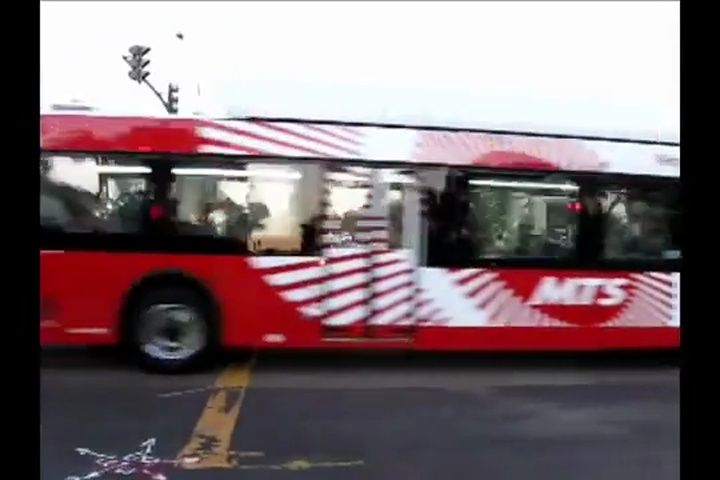
\includegraphics[width=1\linewidth]{a1.jpg}
  %\caption{fig1}
  \end{minipage}%
  }%
  \subfigure[]{
  \begin{minipage}[t]{0.3\linewidth}
  \centering
  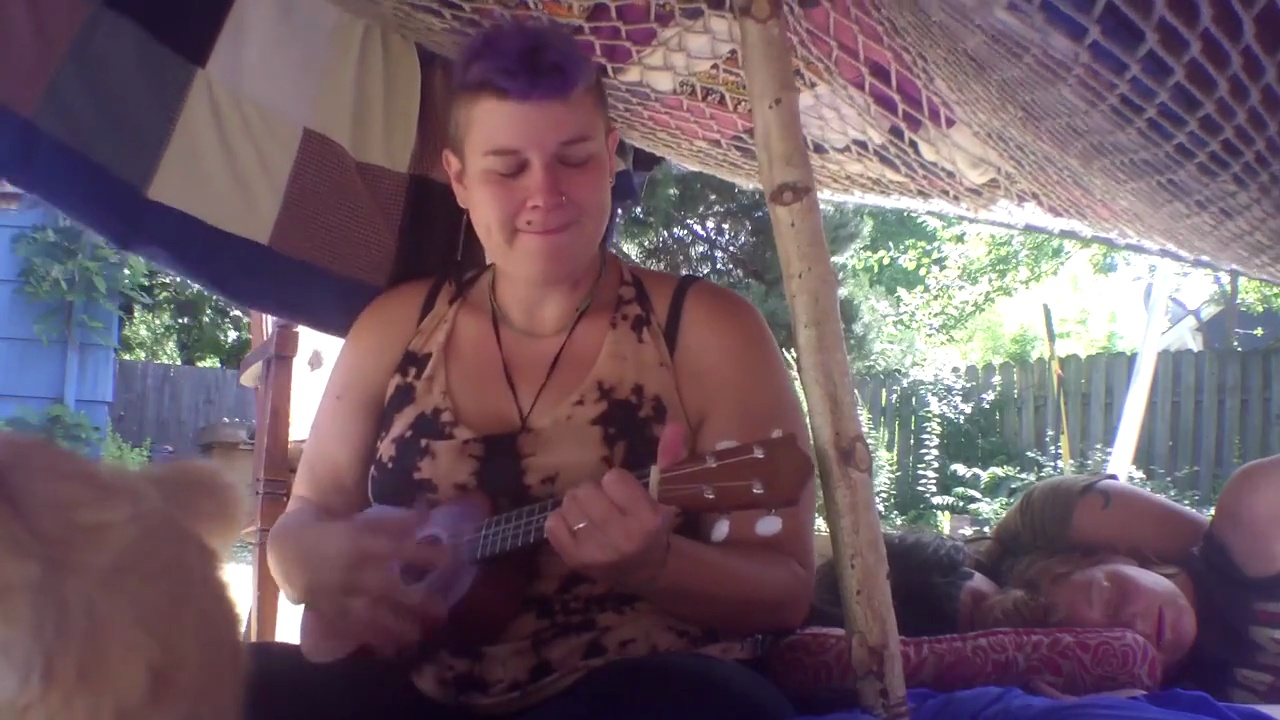
\includegraphics[width=1\linewidth]{a2.jpg}
  %\caption{fig2}
  \end{minipage}%
  }%
  \subfigure[]{
  \begin{minipage}[t]{0.3\linewidth}
  \centering
  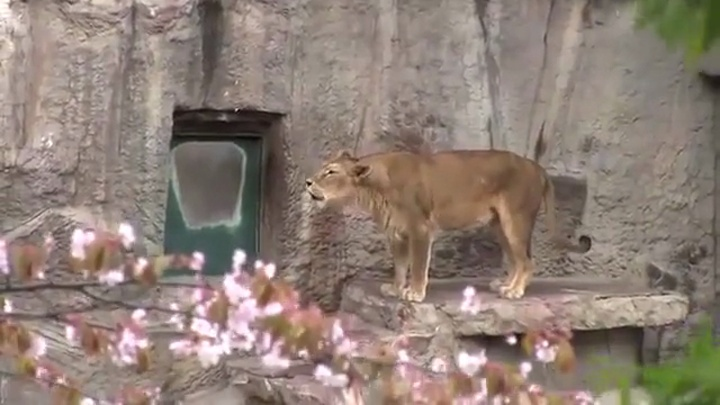
\includegraphics[width=1\linewidth]{a3.jpg}
  %\caption{fig2}
  \end{minipage}%
  }%

  \subfigure[]{
  \begin{minipage}[t]{0.3\linewidth}
  \centering
  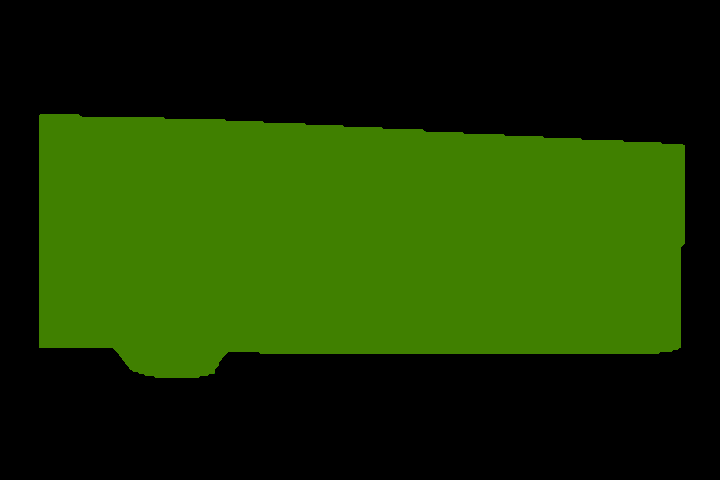
\includegraphics[width=1\linewidth]{a1.png}
  %\caption{fig1}
  \end{minipage}%
  }%
  \subfigure[]{
  \begin{minipage}[t]{0.3\linewidth}
  \centering
  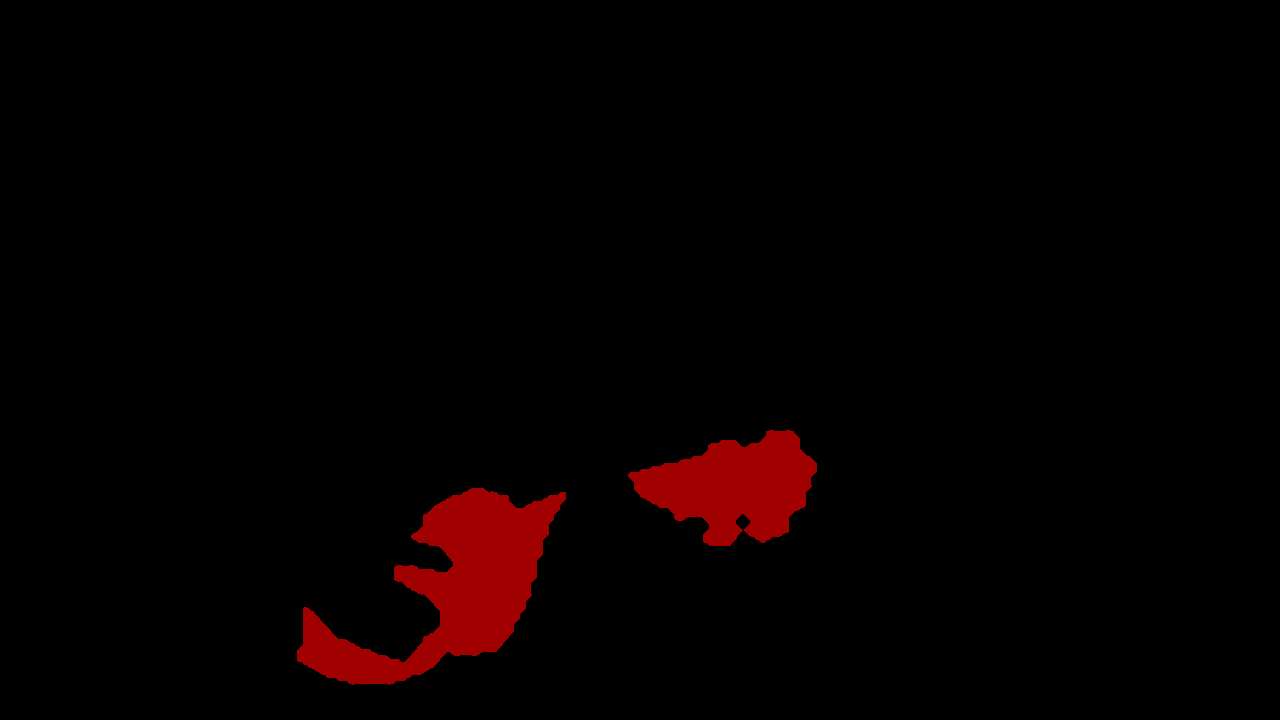
\includegraphics[width=1\linewidth]{a2.png}
  %\caption{fig2}
  \end{minipage}%
  }%
  \subfigure[]{
  \begin{minipage}[t]{0.3\linewidth}
  \centering
  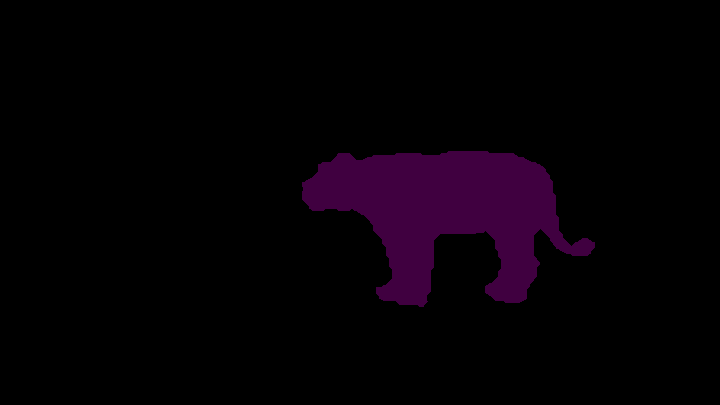
\includegraphics[width=1\linewidth]{a3.png}
  %\caption{fig2}
  \end{minipage}%
  }%
  \caption{AVSBench中的一些样本。(a)-(c)为图片,(d)-(f)为掩码标注。}
\label{fig:avs}
\end{figure}
\paragraph{VGGSound 10K} VGGSound 10K为声源定位领域的Benchmark之一,是从VGGSound数据集中采样10K个样本得到,每个样本的声源标注为边界框,如图\ref{fig:vgg}。由于每个视频样本的时长不同,我们只取了每个视频的第一帧和中间3s的音频用于训练和测试,经过STFT提取频谱图为pkl文件以作为模型输入。EZVSL提供的VGGSound 10K的ID文件只能找到7千多条对应视频,我们从VGGSound中又采样了两千多条视频填充为10K条。
\begin{figure}[!h]
  \centering
  \subfigure[]{
  \begin{minipage}[t]{0.3\linewidth}
  \centering
  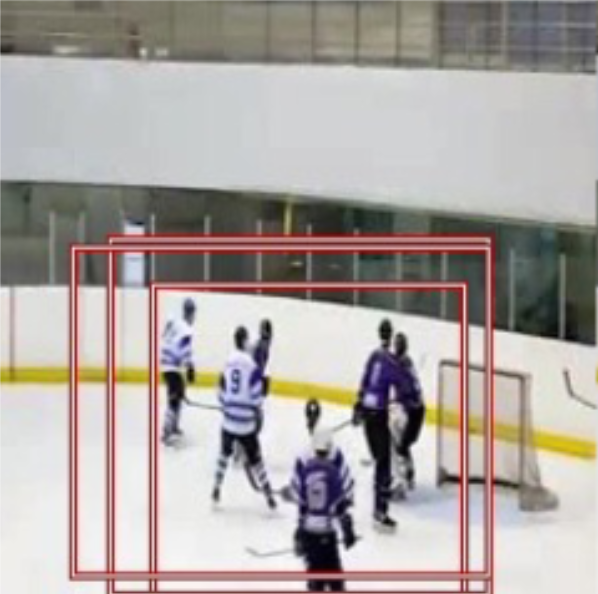
\includegraphics[width=1\linewidth]{v1.png}
  %\caption{fig1}
  \end{minipage}%
  }%
  \subfigure[]{
  \begin{minipage}[t]{0.3\linewidth}
  \centering
  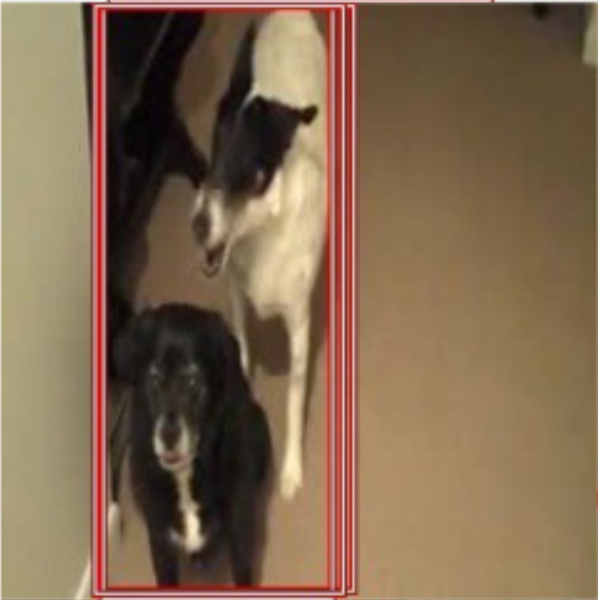
\includegraphics[width=1\linewidth]{v2.png}
  %\caption{fig2}
  \end{minipage}%
  }%
  \subfigure[]{
  \begin{minipage}[t]{0.3\linewidth}
  \centering
  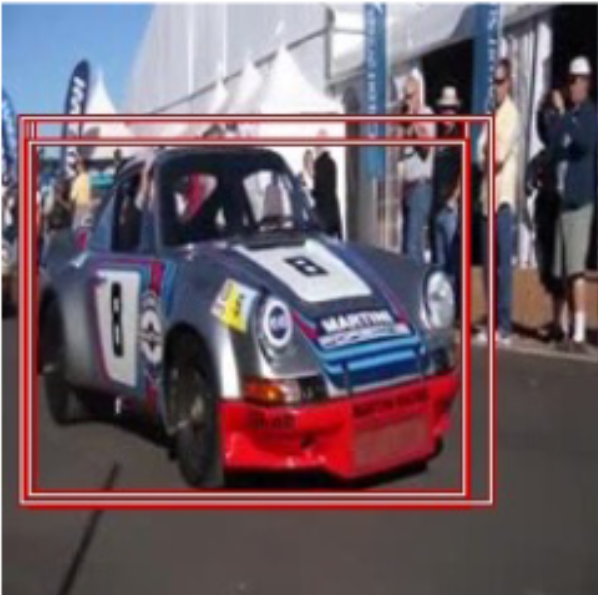
\includegraphics[width=1\linewidth]{v3.png}
  %\caption{fig2}
  \end{minipage}%
  }%
  \caption{VGGSound 10K中的一些样本及其标注。}
\label{fig:vgg}
\end{figure}
\subsection{优化思路}
正如上一部分所说,GSAVL模型的主要结构为声源定位模型+prompt采样器+SAM,其中SAM的参数是固定的,我们主要针对声源定位模型和prompt采样器这两部分进行优化。对于声源定位模型,我们以EZ-VSL为baseline,在VGGSound 10K上进行实验,主要对语音编码器和相似度度量函数进行优化,并进行了消融实验验证有效性,见\ref{vsl};对于采样器,我们在AVSBench上测试了设计的几个采样器的效果,见\ref{samplerex}。

\subsection{结果对比}
在AVSBench上,GSAVL和EZVSL的精度如表\ref{figure:com1}所示,我们的模型在具有分割精度的声源定位数据集上远超传统声源定位模型,究其原因,在于过去的SSL模型只能模糊给出发声区域,而对声源的边界、大小没有感知,因此在需要shape-aware的数据集上效果较差。
\begin{table}[H]
    \centering
    \begin{tabular}{|c|c|}
    \hline
         模型 &  测试集IoU(\%) \\ \hline
        EZVSL &  30.22 \\ \hline
        GSAVL(Ours)&\textbf{48.84}\\\hline
    \end{tabular}
    \caption{AVSBench数据集的结果对比}
    \label{figure:com1}
\end{table}
在VGGSound上,我们测试了优化后的声源定位模型(图\ref{refmodel1})与EZVSL在传统SSL数据集上的性能,结果如表所示验证了我们做出的优化的有效性。
\begin{table}[H]
    \centering
    \begin{tabular}{|c|c|}
    \hline
         模型 &  测试集IoU(\%) \\ \hline
        EZVSL &  36.67 \\ \hline
        Ours&\textbf{37.23}\\\hline
    \end{tabular}
    \caption{VGGSound数据集的结果对比}
    \label{figure:com2}
\end{table}
\subsection{声源定位模型}\label{vsl}

\begin{table}[H]
  \begin{minipage}[t]{0.3\linewidth}
    \centering
    \begin{tabular}{|l|l|}
  \hline
      编码器 &  测试集IoU(\%) \\ \hline
      ResNet18 &  36.67 \\ \hline
      VGGish &  36.75 \\ \hline
  \end{tabular}
  \caption{语音编码器对比}
  \label{table1}
  \end{minipage}%
  \begin{minipage}[t]{0.3\linewidth}
    \centering
    \begin{tabular}{|l|l|}
    \hline
        相似度度量 &  测试集IoU(\%) \\ \hline
        点积 &  36.67 \\ \hline
        余弦相似度&36.94\\\hline
    \end{tabular}
    \caption{相似度度量对比}
    \label{table2}
  \end{minipage}
  \begin{minipage}[t]{0.3\linewidth}
    \centering
    \begin{tabular}{|l|l|}
    \hline
        模型 &  测试集IoU(\%) \\ \hline
        baseline &  36.67 \\ \hline
        VGGish&36.75\\\hline
        余弦相似度&36.94\\\hline
        GSAVL&37.23\\\hline
    \end{tabular}
    \caption{消融实验}
    \label{table3}
  \end{minipage}
\end{table}
\paragraph{语音编码器的选择}
EZVSL中使用的语音编码器为ResNet,我们遵循一些其他的工作,将语音编码器换为VGGish,并在其之后加入线性层,将语音特征与视觉特征统一到同一个特征空间,后者在较大的语音数据集上进行过预训练,相当于语音任务中的backbone。实验结果如表\ref{table1}所示,有较小的提升。
\paragraph{相似度衡量的选择}
EZVSL中使用点积作为视觉和语音特征之间的相似度度量,我们在实验中发现这种方式的结果不稳定,因此在点积前加入了归一化,相当于使用余弦相似度来衡量。实验结果如表\ref{table2}所示,有较大的提升。

\paragraph{消融实验}
对于语音编码器和相似度度量的优化,我们设计了消融实验,进一步检验他们的效果。在GSAVL中,我们既使用VGGish作为语音编码器,又使用余弦相似度衡量视觉和语音特征的对应,如表\ref{table3}所示,两种模块相比 baseline 均提升了精度,并且二者结合使精度进一步提高,证明了他们都是有效的。

\subsection{采样器}\label{samplerex}
我们测试了不同类型采样器的效果,如表\ref{figure:sampler}所示,与声源定位模型baseline相比,我们的方法均实现了提升,其中概率采样方法的精度最高。
\begin{table}[H]
    \centering
    \begin{tabular}{|c|c|}
    \hline
         采样器 &  测试集IoU(\%) \\ \hline
         baseline &  30.22 \\ \hline
        朴素采样 &  34.26 \\ \hline
        网格采样&40.66\\\hline
        概率采样&48.84\\\hline
    \end{tabular}
    \caption{采样器的选择}
    \label{figure:sampler}
\end{table}
\subsection{零样本泛化}
由于声源分割领域只有AVSBench一个benchmark,定量测试模型的零样本泛化能力并不容易,因此,我们将在本部分进行定性的分析。我们在VGGSound数据集中,人工挑选了一些AVSBench中没有的出现过的声源类型数据,并使用在AVSBench数据集上训练的GSAVL模型进行推理,效果如图所示\ref{ref:z1}。根据AVSBench的元数据文件,其中并不含挖掘机、闹钟、猪和乒乓球桌的声源类,但我们的模型仍可以定位并将声源的形状预测的较为精准。
\begin{figure}[!h]
  \centering
  \subfigure[]{
  \begin{minipage}[t]{0.2\linewidth}
  \centering
  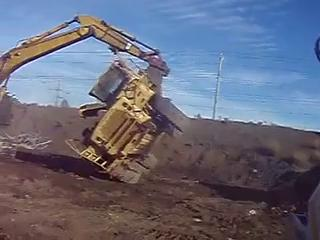
\includegraphics[width=1\linewidth]{z2.jpg}
  %\caption{fig1}
  \end{minipage}%
  \begin{minipage}[t]{0.2\linewidth}
  \centering
  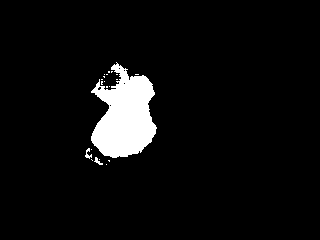
\includegraphics[width=1\linewidth]{zs2.png}
  %\caption{fig1}
  \end{minipage}%
  }%
  \subfigure[]{
 \begin{minipage}[t]{0.2\linewidth}
  \centering
  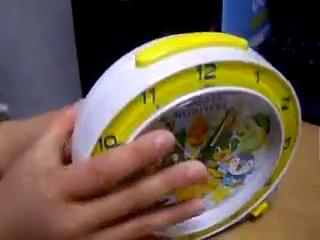
\includegraphics[width=1\linewidth]{z3.jpg}
  %\caption{fig1}
  \end{minipage}%
  \begin{minipage}[t]{0.2\linewidth}
  \centering
  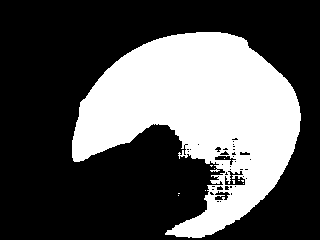
\includegraphics[width=1\linewidth]{zs3.png}
  %\caption{fig1}
  \end{minipage}%
  }%

  \subfigure[]{
  \begin{minipage}[t]{0.2\linewidth}
  \centering
  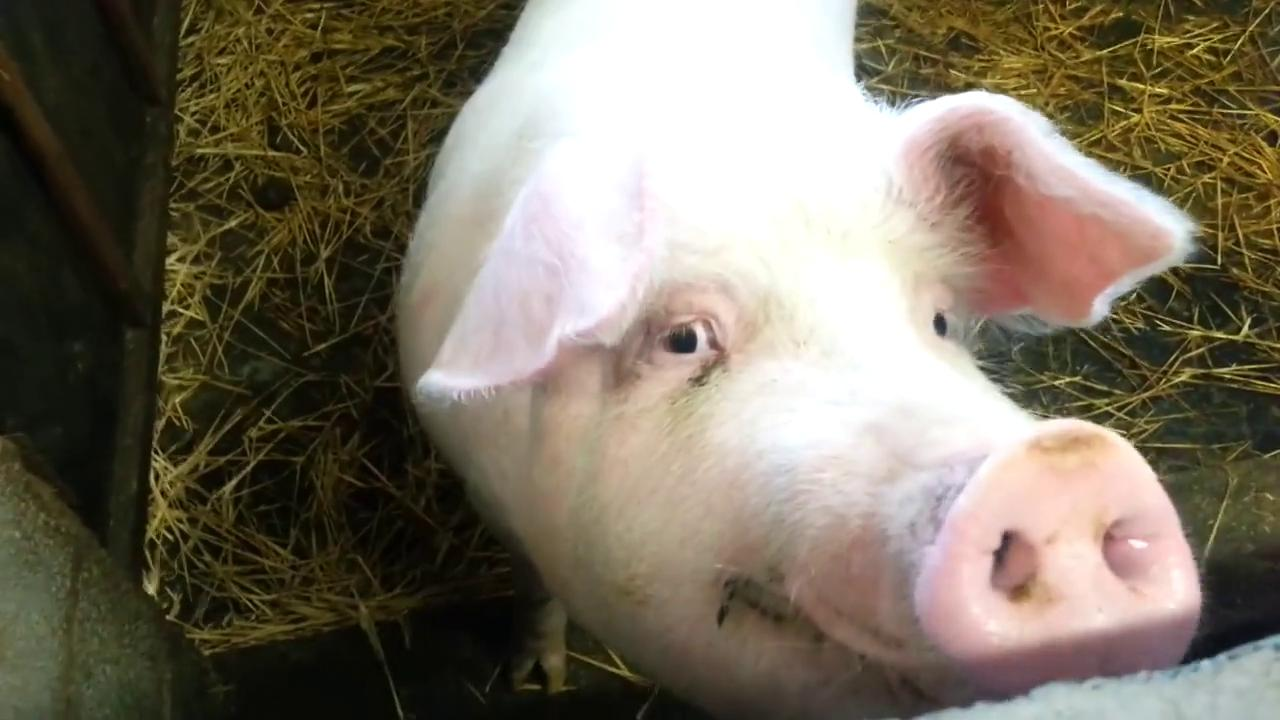
\includegraphics[width=1\linewidth]{z4.jpg}
  %\caption{fig1}
  \end{minipage}%
  \begin{minipage}[t]{0.2\linewidth}
  \centering
  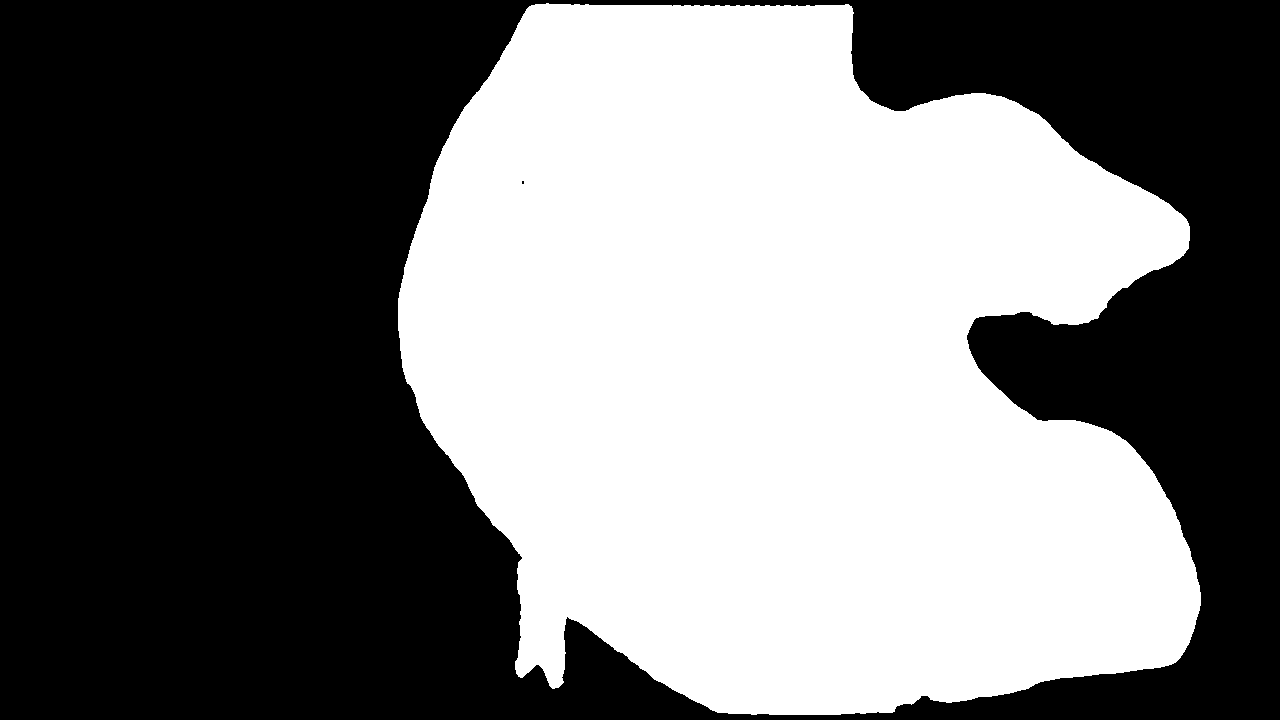
\includegraphics[width=1\linewidth]{zs4.png}
  %\caption{fig1}
  \end{minipage}%
  }%
  \subfigure[]{
 \begin{minipage}[t]{0.2\linewidth}
  \centering
  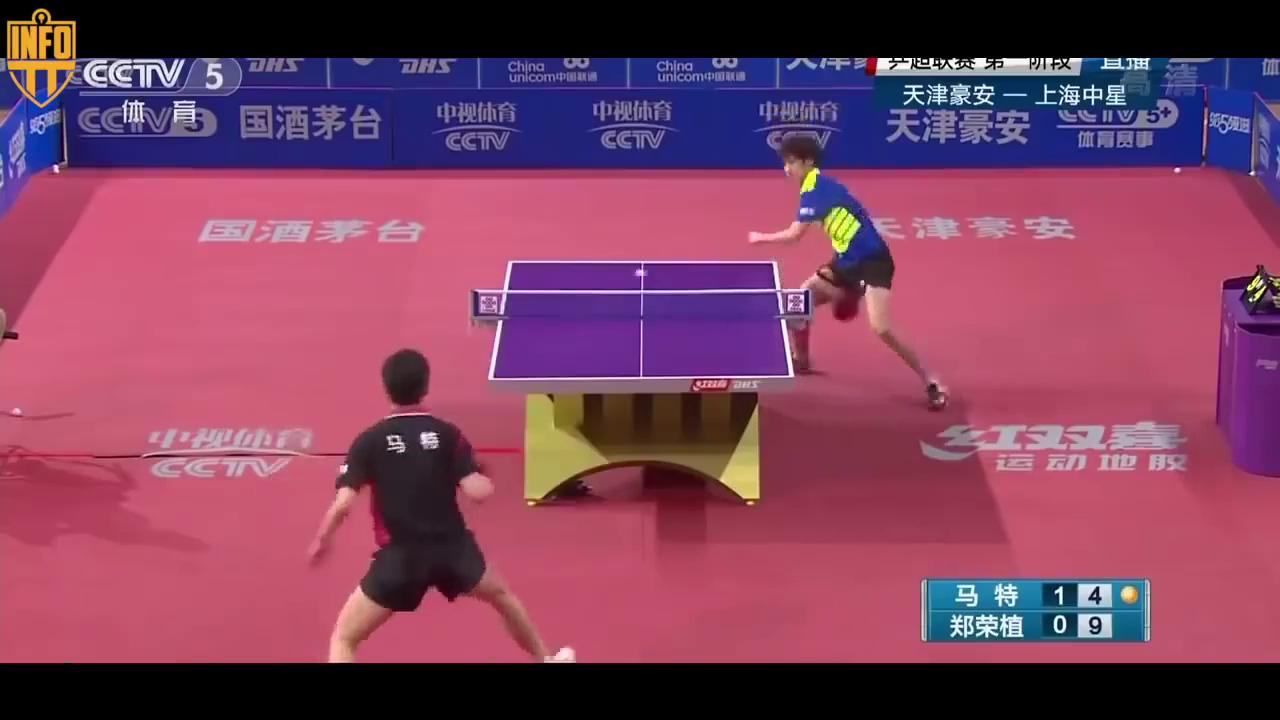
\includegraphics[width=1\linewidth]{z5.jpg}
  %\caption{fig1}
  \end{minipage}%
  \begin{minipage}[t]{0.2\linewidth}
  \centering
  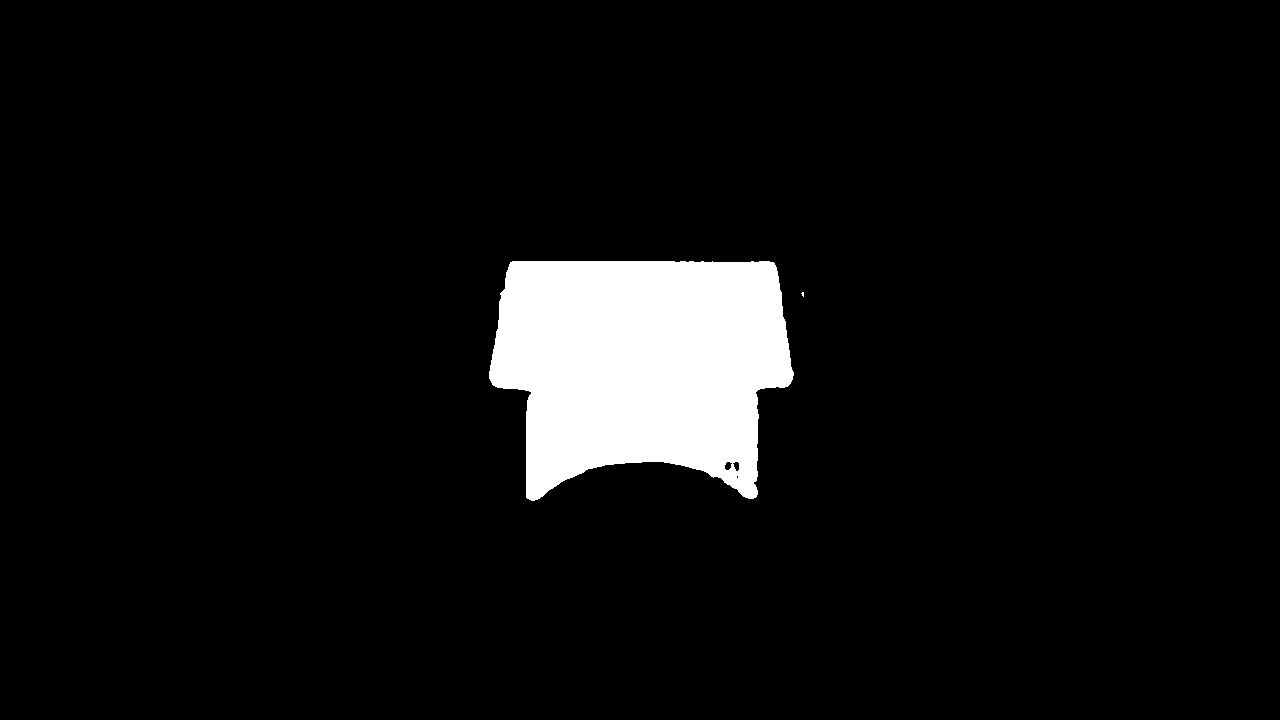
\includegraphics[width=1\linewidth]{zs5.png}
  %\caption{fig1}
  \end{minipage}%
  }%
  \centering
  \caption{在VGGSound上测试零样本泛化能力的结果。}
  \label{ref:z1}
\end{figure}

在我们看来,GSAVL泛化性能力的来源主要分为两部分。一方面为,在大型但模态数据集上预训练的特征提取器,ResNet和VGGish的预训练数据中有大量AVS数据集中未见过的语义类,在GSAVL的自监督训练过程中,视觉与音频的特征空间对齐,使得未见过的类特征也会被拉进,比如说,若某一未见类别i在视觉特征空间中与训练集中的类别j邻近,如果在语音空间i也靠近j,那么模型即使未见过类别i,仍可将该声源定位出来。另一方面为,SAM强大的零样本泛化能力,即使模型从未见过的声源类,只要声源定位模型给出较精确的定位结果,SAM就可以把它的形状很好的分割出来。
\subsection{失败尝试}
我们在这一个月里还尝试了许多可能的优化,例如,改变视觉编码器的结构,将视觉特征图由7*7升为14*14,进而提高定位的精度,但是效果并不理想。

另外,为了保证图片的全局语义与音频特征表征的语义对齐,我们尝试加入一个视音语义对齐损失,先将视觉特征图$f_v^i$最大池化得到$\hat{f_v^i}$,表征视觉的全局语义特征,并希望该特征与语音特征对齐,具体形式为,
\begin{equation}
    \hat{f_v^i}=GMP(f_v^i)
\end{equation}
\begin{equation}
        L_{glo}^i=-log(softmax_v(<\hat{f_v^i},f_a^j>)-log(softmax_a(<f_a^i,\hat{f_v^j}>))
\end{equation}
使用的总损失如下
\[L=L_{a->v}+L_{v->a}+\beta L_{glo}\]
$\beta$为权衡两种损失的超参数。

实验结果如表\ref{tab:my_label}所示,该损失确实可以带来效果的提升,并且与VGGish的消融实验也有效,但是在最后三个优化加一起的消融实验中,精度反而下降,不如GSAVL,因此我们最终没有加入该损失项。

\begin{table}[H]
    \centering
    \begin{tabular}{|c|c|}
    \hline
         模型 &  测试集IoU(\%) \\ \hline
        baseline &  36.67 \\ \hline
        语义对齐损失&37.02\\\hline
        VGGish+语义对齐损失&37.05\\\hline
        视音融合损失+VGGish+余弦相似度&37.16\\\hline
        GSAVL&\textbf{37.23}\\\hline
    \end{tabular}
    \caption{语义对齐损失}
    \label{tab:my_label}
\end{table}
我们较仔细地调节了语义对齐损失的池化方法,和该损失在总损失中的权重项$\beta$,如表\ref{figure:aligh}所示,其中$\beta$=2时使用全局最大池化得到最佳效果。
\begin{table}[H]
    \centering
    \begin{tabular}{|c|c|c|}
    \hline
         池化方法&$\beta$ &  测试集IoU(\%) \\ \hline
        GMP &0.1&  36.65 \\ \hline
        GMP &1&  36.82 \\ \hline
        GMP &2&  37.02 \\ \hline
        GMP &5&  36.60 \\ \hline
        GAP &1&  36.29 \\ \hline
    \end{tabular}
    \caption{对于语义对齐损失的尝试}
    \label{figure:aligh}
\end{table}
\section{总结}
\subsection{模型效果展示}
我们选择了AVSBench数据集中测试集的几个样本,对GSAVL的效果进行展示,如图\ref{ref:result}所示,我们省略了输入的音频的展示。
\begin{figure}[!h]
  \centering
  \subfigure[]{
  \begin{minipage}[t]{0.15\linewidth}
  \centering
  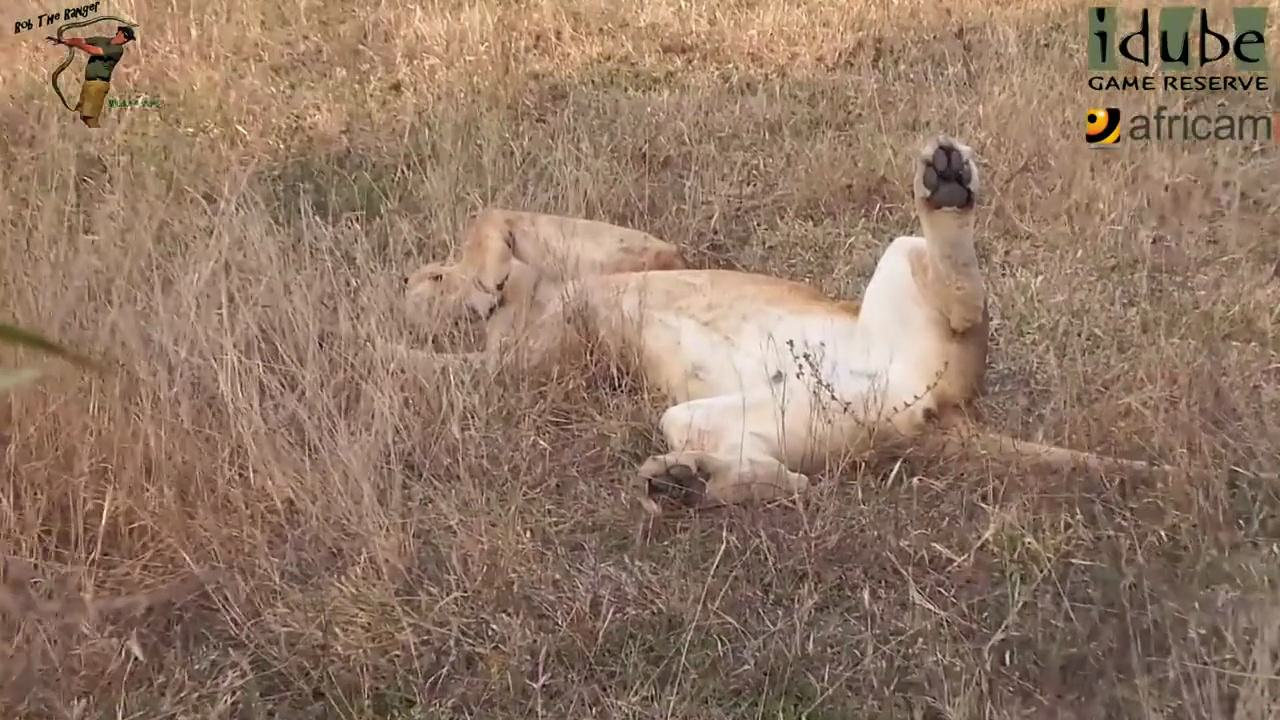
\includegraphics[width=1\linewidth]{84_img.jpg}
  %\caption{fig1}
  \end{minipage}%
  \begin{minipage}[t]{0.15\linewidth}
  \centering
  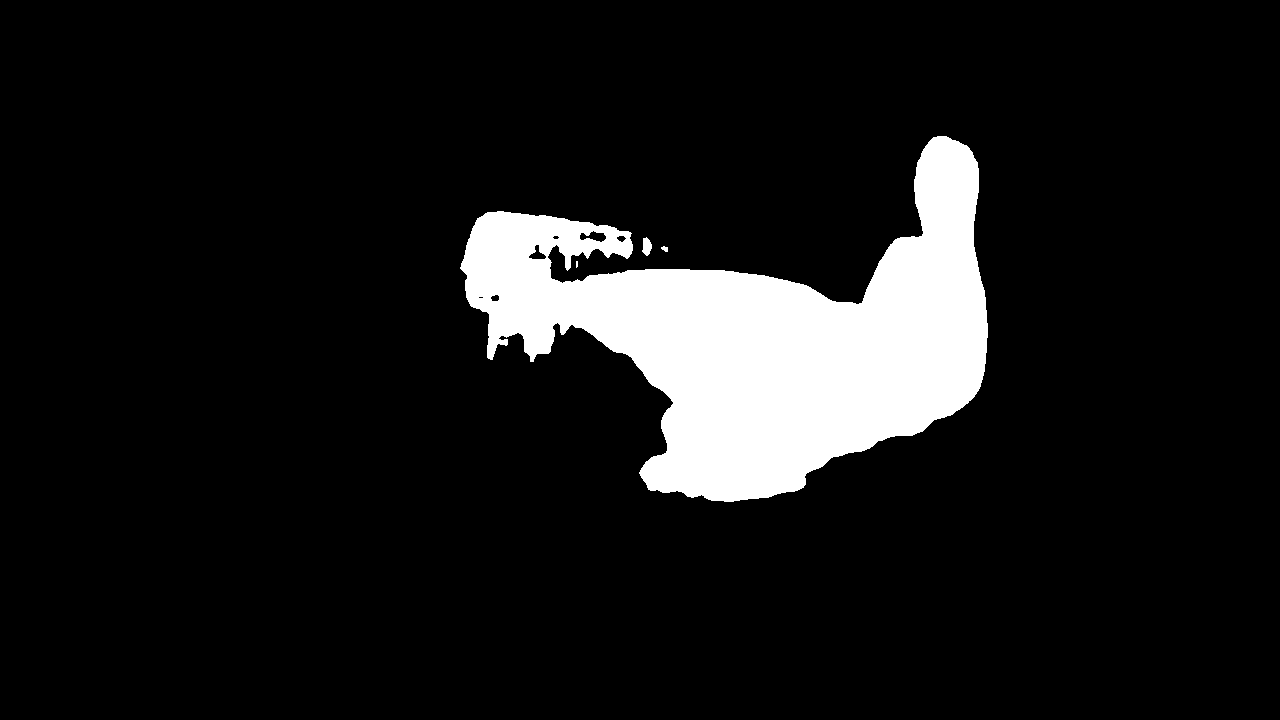
\includegraphics[width=1\linewidth]{84_avobj.png}
  %\caption{fig1}
  \end{minipage}%
  \begin{minipage}[t]{0.15\linewidth}
  \centering
  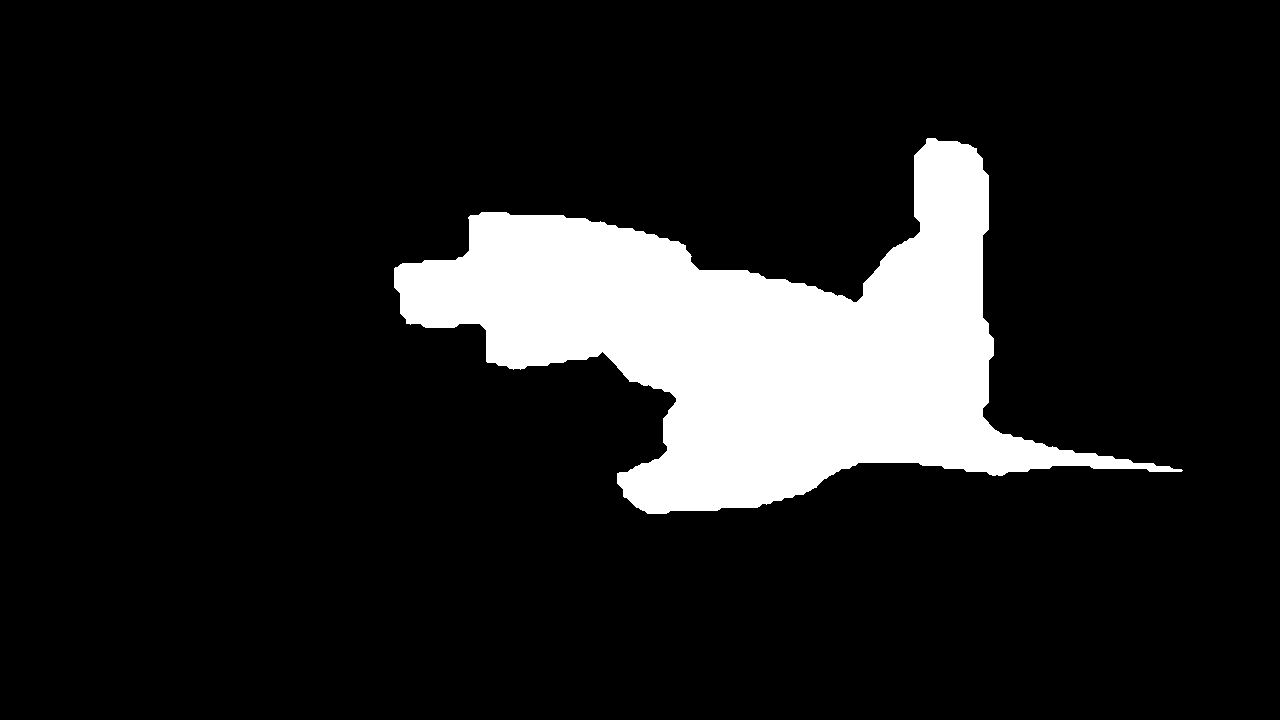
\includegraphics[width=1\linewidth]{84_gt.png}
  %\caption{fig1}
  \end{minipage}%
  }%
  \subfigure[]{
  \begin{minipage}[t]{0.15\linewidth}
  \centering
  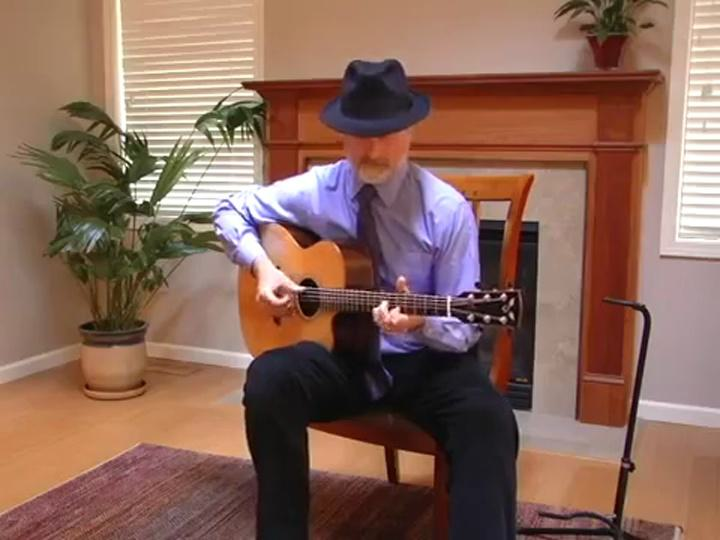
\includegraphics[width=1\linewidth]{90_img.jpg}
  %\caption{fig1}
  \end{minipage}%
  \begin{minipage}[t]{0.15\linewidth}
  \centering
  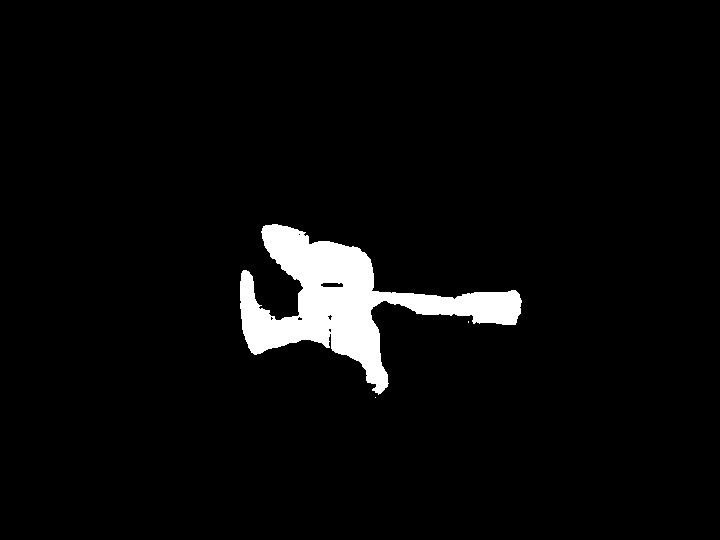
\includegraphics[width=1\linewidth]{90_avobj.png}
  %\caption{fig1}
  \end{minipage}%
  \begin{minipage}[t]{0.15\linewidth}
  \centering
  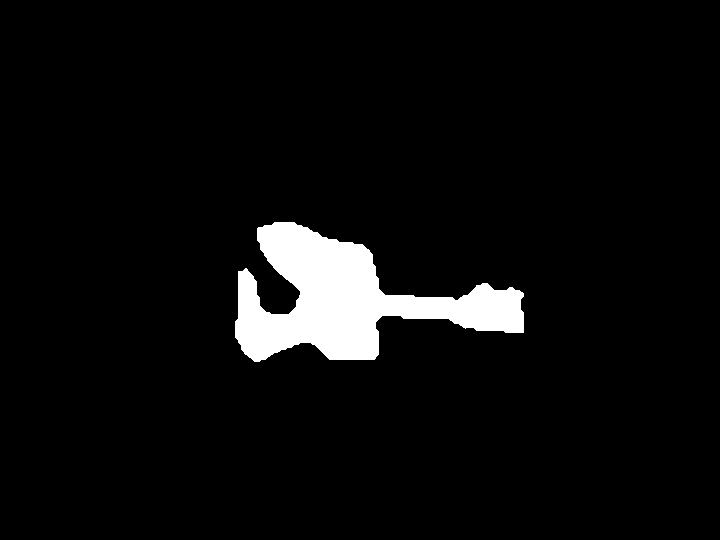
\includegraphics[width=1\linewidth]{90_gt.png}
  %\caption{fig1}
  \end{minipage}%
  }%

  \subfigure[]{
  \begin{minipage}[t]{0.15\linewidth}
  \centering
  \includegraphics[width=1\linewidth]{118_img.jpg}
  %\caption{fig1}
  \end{minipage}%
  \begin{minipage}[t]{0.15\linewidth}
  \centering
  \includegraphics[width=1\linewidth]{118_avobj.png}
  %\caption{fig1}
  \end{minipage}%
  \begin{minipage}[t]{0.15\linewidth}
  \centering
  \includegraphics[width=1\linewidth]{118_gt.png}
  %\caption{fig1}
  \end{minipage}%
  }%
  \subfigure[]{
  \begin{minipage}[t]{0.15\linewidth}
  \centering
  \includegraphics[width=1\linewidth]{97_img.jpg}
  %\caption{fig1}
  \end{minipage}%
  \begin{minipage}[t]{0.15\linewidth}
  \centering
  \includegraphics[width=1\linewidth]{97_avobj.png}
  %\caption{fig1}
  \end{minipage}%
  \begin{minipage}[t]{0.15\linewidth}
  \centering
  \includegraphics[width=1\linewidth]{97_gt.png}
  %\caption{fig1}
  \end{minipage}%
  }%

  \subfigure[]{
  \begin{minipage}[t]{0.15\linewidth}
  \centering
  \includegraphics[width=1\linewidth]{128_img.jpg}
  %\caption{fig1}
  \end{minipage}%
  \begin{minipage}[t]{0.15\linewidth}
  \centering
  \includegraphics[width=1\linewidth]{128_avobj.png}
  %\caption{fig1}
  \end{minipage}%
  \begin{minipage}[t]{0.15\linewidth}
  \centering
  \includegraphics[width=1\linewidth]{128_gt.png}
  %\caption{fig1}
  \end{minipage}%
  }%
  \subfigure[]{
  \begin{minipage}[t]{0.15\linewidth}
  \centering
  \includegraphics[width=1\linewidth]{168_img.jpg}
  %\caption{fig1}
  \end{minipage}%
  \begin{minipage}[t]{0.15\linewidth}
  \centering
  \includegraphics[width=1\linewidth]{168_avobj.png}
  %\caption{fig1}
  \end{minipage}%
  \begin{minipage}[t]{0.15\linewidth}
  \centering
  \includegraphics[width=1\linewidth]{168_gt.png}
  %\caption{fig1}
  \end{minipage}%
  }%
  \centering
  \caption{结果展示。每个子图的第一张为原图,第二张为GSAVL的结果,第三张为真值掩码。}
  \label{ref:result}
\end{figure}
\subsection{现存问题分析}\label{ques}
如上一部分所示,GSAVL在测试集上的大部分样本都取得了较好的结果,但经过我们分析模型的预测结果,发现了以下现存的问题,模型仍然具有改进空间。

\paragraph{模型鲁棒性}
尽管已经在prompt的学习上考虑了鲁棒性,但是我们的方法仍较强的依赖于自监督声源定位模型的效果。当声源定位模型给出的定位热力图精度较差,特别是极值点未落在声源上时,如图\ref{ref:x1}所示,甚至会出现将非声源部分完全分割出来的结果。(a),(b),(c)的例子中,由于定位图的精度问题,prompt采样到了马旁边的栏杆上,导致SAM的分割结果与声源背道而驰。

我们想到了一种较简单的方法来避免这种情况,但是这种方法对计算资源的要求较高,我们还没来得及实现。我们认为可以尝试一种级联细化的方法,根据前一次迭代得到的SAM预测mask,计算其与声源定位图的相似度/JS散度,如果相似度高于某一阈值,则认为学习到的prompt成功将声源指出来,否则,重新采样prompt,重新输入SAM预测,直到相似度高于阈值,或达到某一最大迭代次数。
\begin{figure}[!h]
  \centering
  \subfigure[]{
  \begin{minipage}[t]{0.3\linewidth}
  \centering
  \includegraphics[width=1\linewidth]{30_img.jpg}
  %\caption{fig1}
  \end{minipage}%
  }%
  \subfigure[]{
  \begin{minipage}[t]{0.3\linewidth}
  \centering
  \includegraphics[width=1\linewidth]{30_avobj.png}
  %\caption{fig1}
  \end{minipage}%
  }%
  \subfigure[]{
  \begin{minipage}[t]{0.3\linewidth}
  \centering
  \includegraphics[width=1\linewidth]{30_gt.png}
  %\caption{fig1}
  \end{minipage}%
  }%

  \subfigure[]{
  \begin{minipage}[t]{0.3\linewidth}
  \centering
  \includegraphics[width=1\linewidth]{40_img.jpg}
  %\caption{fig1}
  \end{minipage}%
  }%
  \subfigure[]{
  \begin{minipage}[t]{0.3\linewidth}
  \centering
  \includegraphics[width=1\linewidth]{40_avobj.png}
  %\caption{fig1}
  \end{minipage}%
  }%
  \subfigure[]{
  \begin{minipage}[t]{0.3\linewidth}
  \centering
  \includegraphics[width=1\linewidth]{40_gt.png}
  %\caption{fig1}
  \end{minipage}%
  }%

  \centering
  \caption{模型鲁棒性的样例研究。第一列为原图,第二列为GSAVL的结果,第三列为真值掩码。}
  \label{ref:x1}
\end{figure}
\paragraph{SAM的歧义性}
SAM的歧义性在原论文中便被提出,当prompt落在图片上的一个点,该点所在的目标可能有多种可能的语义对象,引发掩码预测的歧义性。如图\ref{ref:x2}所示,尽管声源定位模型给出了足够精确的定位,提取的prompt落在了声源上,但是效果并不符合期望,(a)行的prompt落在了键盘的一个按钮上,我们期望SAM将整个键盘分割出来,但是最后只分割出来了那一个按钮;(b)行的prompt落在人的头发上,我们期望SAM将人分割出来,但是最后只分割出来了头发部分;(c)行的prompt落在除草机的铁盖上,我们期望SAM将整个除草机分割出来,但最后只分割出来了铁盖那一部分。
\begin{figure}[!h]
  \centering
  \subfigure[]{
  \begin{minipage}[t]{0.3\linewidth}
  \centering
  \includegraphics[width=1\linewidth]{45_img.jpg}
  %\caption{fig1}
  \end{minipage}%
  }%
  \subfigure[]{
  \begin{minipage}[t]{0.3\linewidth}
  \centering
  \includegraphics[width=1\linewidth]{45_avobj.png}
  %\caption{fig1}
  \end{minipage}%
  }%
  \subfigure[]{
  \begin{minipage}[t]{0.3\linewidth}
  \centering
  \includegraphics[width=1\linewidth]{45_gt.png}
  %\caption{fig1}
  \end{minipage}%
  }%

  \subfigure[]{
  \begin{minipage}[t]{0.3\linewidth}
  \centering
  \includegraphics[width=1\linewidth]{48_img.jpg}
  %\caption{fig1}
  \end{minipage}%
  }%
  \subfigure[]{
  \begin{minipage}[t]{0.3\linewidth}
  \centering
  \includegraphics[width=1\linewidth]{48_avobj.png}
  %\caption{fig1}
  \end{minipage}%
  }%
  \subfigure[]{
  \begin{minipage}[t]{0.3\linewidth}
  \centering
  \includegraphics[width=1\linewidth]{48_gt.png}
  %\caption{fig1}
  \end{minipage}%
  }%

\subfigure[]{
  \begin{minipage}[t]{0.3\linewidth}
  \centering
  \includegraphics[width=1\linewidth]{61_img.jpg}
  %\caption{fig1}
  \end{minipage}%
  }%
  \subfigure[]{
  \begin{minipage}[t]{0.3\linewidth}
  \centering
  \includegraphics[width=1\linewidth]{61_avobj.png}
  %\caption{fig1}
  \end{minipage}%
  }%
  \subfigure[]{
  \begin{minipage}[t]{0.3\linewidth}
  \centering
  \includegraphics[width=1\linewidth]{61_gt.png}
  %\caption{fig1}
  \end{minipage}%
  }%
  \centering
  \caption{SAM歧义性的样例研究。第一列为原图,第二列为GSAVL的结果,第三列为真值掩码。}
  \label{ref:x2}
\end{figure}

其实,SAM已给出了应对歧义的解决方案,可以将SAM的multimask\_output设为True,SAM会对不明确的输入prompt,在考虑歧义的情况下返回多个预测掩码,其中每个掩码对应一个可能的语义对象。但是,由于我们无监督的任务设置,较难在多个预测掩码中,选择最佳掩码,因此我们设置了multimask\_output为False。


\paragraph{数据集的偏差}
在我们分析预测样例的过程中,发现AVSBench数据集的真值掩码有偏差,如图\ref{ref:x3}所示,GSAVL的结果明显将声源“猫”很好的分割出来,但是该图的真值掩码(C)与真实的分割有一定的偏差,引起计算精度较低。
\begin{figure}[!h]
  \centering
  \subfigure[]{
  \begin{minipage}[t]{0.3\linewidth}
  \centering
  \includegraphics[width=1\linewidth]{56_img.jpg}
  %\caption{fig1}
  \end{minipage}%
  }%
  \subfigure[]{
  \begin{minipage}[t]{0.3\linewidth}
  \centering
  \includegraphics[width=1\linewidth]{56_avobj.png}
  %\caption{fig1}
  \end{minipage}%
  }%
  \subfigure[]{
  \begin{minipage}[t]{0.3\linewidth}
  \centering
  \includegraphics[width=1\linewidth]{56_gt.png}
  %\caption{fig1}
  \end{minipage}%
  }%
  \centering
  \caption{数据集的偏差。第一列为原图,第二列为GSAVL的结果,第三列为真值掩码。}
  \label{ref:x3}
\end{figure}

\subsection{可执行代码构成}
我们提交的代码(GSAVL文件夹)是可以执行的,但是不能直接执行,因为提交的文件夹内没有放SAM和VGGish的预训练权重,这两个太大了,其中,SAM应下载以ViT-h为主干的checkpoint,并放在models/segment\_anything/checkpoint路径下,VGGish的预训练权重应放在"models/vggish"下,下面将简单介绍一下我们代码中每个文件和文件夹的作用。

\textit{audio_io.py,exact_spec_vgg.py,utils.py里为一些工具函数/类,包括读取音频,提取音频的频谱图,记录实验结果,保存日志等功能.}

\textit{model.py为模型文件,train.py,test.py和dataset.py分别为我们实现的训练、测试框架,和使用的数据集设置,config.py为一些配置,其中的数据集路径等设置应按实际情况修改。}

\textit{demo.py为我们实现的一个演示文件,可以方便的推理一个视频的声源,只需在代码前几行更改图片和音频频谱图的路径;在example文件夹下,我们提供了两个图片-频谱图对以供测试。}

\textit{scripts文件夹下为我们的sh脚本文件,可直接运行相应文件执行相应训练/测试;metadata下为一些数据集的元数据。}

\textit{models文件夹下有多个模型,包括SAM源代码(我们做了部分修改),VGGish源代码,EZVSL源代码,和我们的模型GSAVL.}

\textit{checkpoints下存有我们所有在报告中提到的实验对应的训练/测试日志,可按照文件名查阅,其中,我们在train_avs_gsavl下提供了GSAVL在AVSBench数据集上训练的checkpoint以供测试。}

\subsection{总结与展望}
我们小组认为,视频数据将会在未来越发受到社区的关注,出于对Audio-visual领域的兴趣,我们在最初便选定了声源定位作为课程作业的目标。在广泛阅读了声源定位领域的顶会,和新任务声源分割近一年的工作后,我们发现SAM和一些LLM、VLM大模型已经在Audio-visual领域得到应用,因而萌生了将声源定位任务与SAM结合的想法,希望在无监督设置下,利用视觉和声音在时空上的自然对应,进行自监督学习,并利用SAM的强大能力实现具有shape-aware,对声源形状敏感的可泛化的声源定位模型。

经过一个月的努力,我们首先对过去的声源定位模型进行了优化,通过改进语音编码器,优化相似度度量方法,我们训练出了在传统声源定位任务上效果更强,泛化性更强的模型(图\ref{refmodel1})。接着,我们搭建了包含SAM的测试pipeline,并探索了prompt learning的方法,最终实现了概率采样,兼顾鲁棒性,在测试集上达到最佳效果。遗憾的是,如\ref{ques}中所说,我们想到了一种更合适的pipeline,通过级联细化声源定位的结果,但囿于计算资源和时间不足(当前方法对测试集推理一遍需要6小时,级联方法大概会超过12小时),我们尚未尝试该想法。

在这个过程中,我们收获颇多。我们广泛地阅读论文,并在过程中整理论文笔记,在书写报告的相关工作时,我们重新回顾读过的论文,回过头来思考,将方法进行归类,使我们对SSL相关工作的理解进一步提升。我们从零开始设计实验,来验证各种方法的有效性,为了保证对比的充分性和公平性,我们在最后一周还重做和补做了许多实验。我们一张一张分析模型的预测结果,查找现有问题并进行优化,在这个过程中对Audio-visual learning的理解进一步加深。

在报告的最后,正如\ref{ques}所说,我们目前的方法还存在改进空间,在未来的工作中,我们将
在以下方向进行探索

\textit{i)将GSAVL的SAM预测头实现级联结构,迭代细化SAM预测结果,使模型鲁棒性进一步增强,降低对定位预测图极值点的依赖}

\textit{ii)进一步改进声源定位基础模型,我们发现,现有模型在自监督训练时很容易过拟合,需要根据验证集精度人工进行early stop,尽管\cite{23}已经探索了该问题,但尚未很好的解决。}

\textit{iii)相比声源定位任务,声源分割是一个具有挑战性的新任务,我们将在未来持续关注该领域的进一步发展。}
\subsection{小组分工}
马俊程:设计方法,设计实验方案,实现代码框架,完成技术报告的绝大部分,录制演示视频,制作PPT并在研讨课汇报。

张誉丰:探索采样器的实现方式,完成采样器相关实验,完成报告3.4部分。

魏昕原:探索声源定位模型的优化方法,完成部分实验,绘制模型示意图。

宁钰成:探索声源定位模型的优化方法,完成部分实验,绘制模型示意图。
\bibliographystyle{plain}
\bibliography{cite}
\end{document}